\chapter[Annexes]{Annexes}

\localtableofcontents

% \addcontentsline{toc}{chapter}{Annexes}

\chaptermark{Annexes}

%%%%%%%%%%%%%%%%%%%%%%%%%%%%%%%%%%
\section{Proofs in Chapter 1}

\subsection{Unbalanced Optimal Transport}

%%%%%%%%%%%%%%%%%%%%%%%%%%%%%%%%%%%%%%%%%%%%%%
\begin{proof}[Proof of \Cref{coro:uot_l2_mm}]
Note that we can write Problem \eqref{uot_l2} as
\begin{align}
    \min_{t \in \bbR^{mn}_{\geq 0}} \langle c, t \rangle + \frac{|| Mt - y ||^2}{2}
\end{align}
where $t = \vect(P), c = \vect(C)$ are the vectorizations of $P, C$, respectively. Here,
\begin{itemize}
    \item[$\bullet$] $M = (\rho_1^{1/2} M_r^T, \rho_2^{1/2} M_c^T, \varepsilon^{1/2} I_{mn})^T \in \bbR^{(m + n + mn) \times (mn)}$.

    \item[$\bullet$] $y = (\rho_1^{1/2} \mu^T, \rho_2^{1/2} \nu^T, \varepsilon^{1/2} \vect(\gamma)^T)^T \in \bbR^{m + n + mn}$.

    \item[$\bullet$] $M_r = \texttt{np.repeat(np.eye(n),m)} \in \bbR^{n \times mn}$.

    \item[$\bullet$] $M_c = [I_m, ..., I_m] = \texttt{np.tile(np.eye(m),n)} \in \bbR^{m \times mn}$.
\end{itemize}
See Appendix A in \citep{Chapel21} for more details of $M_r, M_c$.
Remark that if $A \in \bbR^{m \times n}$ and $B \in \bbR^{m \times p}$, then
\begin{align}
    (A, B) \begin{pmatrix}
        A^T \\
        B^T
    \end{pmatrix}
    = A A^T + B B^T
\end{align}
Following Equation 23 in \citep{Chapel21},  we have
\begin{align}
    t^{(k+1)}_i = t^{(k)}_i \frac{\max( 0, [M^T y]_i - c_i)}{[M^T M t^{(k)}]_i}
\end{align}
Now, $\text{mat}(M^T y) = (\rho_1 \mu) \oplus (\rho_2 \nu) + \varepsilon \gamma$.
Here, matrization is the inverse operation of vectorization. Also,
$M^T M = \rho_1 M_r^T M_r + \rho_2 M_c^T M_c + \varepsilon I_{mn}$, so
$\text{mat}(M^T M t^{(k)}) = (\rho_1 P_{\# 1}^{(k)}) \oplus (\rho_2 P_{\# 2}^{(k)})
+ \varepsilon P^{(k)} $. The result then follows.
\end{proof}
%%%%%%%%%%%%%%%%%%%%%%%%%%%%%%%%%%%%%%%%%%%%%%

%%%%%%%%%%%%%%%%%%%%%%%%%%%%%%%%%%%%%%%%%%%%%%
\begin{proof}[Proof of \Cref{coro:uot_l2_minimizer}]
We follow the same proof technique of Lemma 4 in \citep{Khiem20}. The $l^2$-squared norm satisfies
$D_{\varphi}(p, q) = \varphi(p) + \varphi(q) - \langle p, q \rangle$. So, for any $t \in \bbR$,
\begin{align}
  \frac{\partial D_{\varphi}(tp, q)}{\partial t}
  &= 2 t \; \varphi(p) - \langle p, q \rangle \\
  &= 2t \left[ \varphi(p) + \varphi(q) - \langle p, q \rangle \right]
  - 2t \; \varphi(q) + (2t-1) \langle p, q \rangle \\
  &= 2t \; D_{\varphi}(p, q) - 2t \; \varphi(q) + (2t - 1) \langle p, q \rangle.
\end{align}
For $t \in \bbR$, denote
\begin{align}
  g(tP) = t^2 \langle C, P \rangle + \rho_1 D_{\varphi}(t P_{\# 1}, \mu) +
  \rho_2 D_{\varphi}(t P_{\# 2}, \nu) + \varepsilon D_{\varphi}(t P, \gamma)
\end{align}
Then, we have
\begin{align}
  \frac{\partial g(tP)}{\partial t} &= 2t \langle C, P \rangle
  + \rho_1 \Big[ 2t \; D_{\varphi}(P_{\# 1}, \mu) - 2t \; \varphi(\mu)
  + (2t - 1) \langle P_{\# 1}, \mu \rangle \Big] \\
  &+ \rho_2 \Big[ 2t \; D_{\varphi}(P_{\# 2}, \nu) - 2t \; \varphi(\nu)
  + (2t - 1) \langle P_{\# 2}, \nu \rangle \Big] \\
  &+ \varepsilon \Big[ 2t \; D_{\varphi}(P, \gamma) - 2t \; \varphi(\gamma)
  + (2t - 1) \langle P, \gamma \rangle \Big] \\
  &= 2t \; g(P) - 2t \Big[ \rho_1 \varphi(\mu)
  + \rho_2 \varphi(\nu) + \varepsilon \varphi(\gamma) \Big] \\
  &+ (2t - 1) \Big[ \rho_1 \langle P_{\# 1}, \mu \rangle
  + \rho_2 \langle P_{\# 2}, \nu \rangle + \varepsilon \langle P, \gamma \rangle \Big]
\end{align}
If $P^*$ is the minimizer, then $\min_{t \in \bbR} g(tP^*) = g(P^*)$ and the minimum is attained
when $t=1$. This means $\frac{\partial g(tP^*)}{\partial t} \Big |_{t = 1} = 0$. So,
\begin{align}
  g(P^*) = \rho_1 \varphi(\mu)
  + \rho_2 \varphi(\nu) + \varepsilon \varphi(\gamma)
  - \frac{1}{2} \Big( \rho_1 \langle P^*_{\# 1}, \mu \rangle
  + \rho_2 \langle P^*_{\# 2}, \nu \rangle + \varepsilon \langle P^*, \gamma \rangle \Big)
\end{align}
The result then follows.
\end{proof}

%%%%%%%%%%%%%%%%%%%%%%%%%%%%%%%%%%%%%%%%%%%%%%
\subsection{Gromov-Wasserstein distance}

%%%%%%%%%%%%%%%%%%%%%%%%%%%%%%%%%%%%%%%%%%%%%%
\begin{corollary}
    The formulations \eqref{GH:zeroth} and \eqref{GH:first} of the Gromov-Hausdorff distance
    are equivalent.
\end{corollary}
\begin{proof}
In the formulation \eqref{GH:first}, by choosing identity mappings (which are clearly isometric embeddings)
$f = \id_X$ and $g = \id_Y$, and $Z = X \cup Y$ equipped with an admissible distance $d$, we have
\begin{equation}
  \gh((X,d_X), (Y,d_Y)) \leq d_{H}^{(Z,d)}(X, Y)
\end{equation}
As this is true for any $d \in \cD(d_X,d_Y)$, we have
$\gh((X,d_X), (Y,d_Y)) \leq \inf_{d} d_{H}^{(X \cup Y, d)}(X, Y)$. For the reverse direction,
given any isometries $f: X \to X'$ and $g: Y \to Y'$ with $X', Y' \subset (Z, d_Z)$
(we call $(X',Y')$ a \textit{metric coupling} \citep{Villani08}), one can define
a distance $d$ on $X \cup Y$ (as shown in Proposition 27.1 in \citep{Villani08}). Then,
\begin{equation}
  \begin{split}
    d_H^{(Z, d_Z)}(f(X), g(Y)) &=
  \max(\sup_{y \in Y} d_Z(g(y), f(X)), \sup_{x \in X} d_Z(f(x), g(Y))) \\
  &= \max(\sup_{y \in Y} d(y, X), \sup_{x \in X} d(x, Y)) \\
  &= d_H^{(X \cup Y, d)}(X, Y) \geq \inf_{d'} d_{H}^{(X \cup Y, d')}(X, Y)
  \end{split}
\end{equation}
We deduce that $\gh((X,d_X), (Y,d_Y)) \geq \inf_{d} d_{H}^{(X \cup Y, d)}(X, Y)$,
thus equality holds.
\end{proof}
%%%%%%%%%%%%%%%%%%%%%%%%%%%%%%%%%%%%%%%%%%%%%%

%%%%%%%%%%%%%%%%%%%%%%%%%%%%%%%%%%%%%%%%%%%%%%
\begin{proof}[Proof of \Cref{lemma:fgw_pgd}]
  Denote $F(P) = \langle C \otimes P, P \rangle + \langle M, P \rangle + \varepsilon \kl(P | \gamma)$.
  Then $\nabla F(P) = C \otimes P + M + \varepsilon \log \frac{P}{\gamma}$.
  The PGD iterate reads: for $\tau > 0$,
  \begin{align}
    P^{(t+1)} = \text{proj}^{\kl}_{U(\mu_x, \mu_y)}
    \left( P^{(t)} \odot e^{-\tau \nabla F(P^{(t)})} \right),
  \end{align}
  where $\text{proj}^{\kl}_{U(\mu_x, \mu_y)}(K) =
  \argmin_{P \in U(\mu_x, \mu_y)} - \varepsilon \langle \log K, P \rangle + \varepsilon H(P)$.
  Denote $\eta = \tau \varepsilon$. We have
  \begin{align}
    \log K &= \log \left( P^{(t)} \odot e^{-\tau \nabla F(P^{(t)})} \right) =
    \log P^{(t)} - \tau (C \otimes P^{(t)} + M)  - \tau \varepsilon \log \frac{P^{(t)}}{\gamma} \\
    &= - \tau (C \otimes P^{(t)} + M) + \log \left( \gamma^{\eta} \odot (P^{(t)})^{1 - \eta} \right)
  \end{align}
  So,
  \begin{align}
    &- \varepsilon \langle \log K, P \rangle + \varepsilon H(P) \\
    &= \eta \langle C \otimes P^{(t)} + M, P \rangle
    - \varepsilon \langle P, \log \left( \gamma^{\eta} \odot (P^{(t)})^{1 - \eta} \right) \rangle
    + \varepsilon H(P) \\
    &= \eta \langle C \otimes P^{(t)} + M, P \rangle +
    \varepsilon \kl \left( P \big | \gamma^{\eta} \odot (P^{(t)})^{1 - \eta} \right)
    - m \left( \gamma^{\eta} \odot (P^{(t)})^{1 - \eta} \right),
  \end{align}
  where $m(Q) = \sum_{i,j} Q_{ij}$ is the mass of measure $Q$. The result then follows.
\end{proof}
%%%%%%%%%%%%%%%%%%%%%%%%%%%%%%%%%%%%%%%%%%%%%%

\subsection{INPUT}
%%%%%%%%%%%%%%%%%%%%%%%%%%%%%%%%%%%%%%%%%%%%%%
\begin{proof}[Proof of \Cref{lemma:convex-smoothness}]
We begin by noticing that $g(\pi) = \kl(\pi | \mu)$ is $1$-strongly convex \wrt the KL divergence.
Indeed, $\nabla g(\pi) = \log \pi - \log \mu$, so for any positive measure $\pi, \gamma$, we have
\begin{align}
    \langle \nabla g(\pi) - \nabla g(\gamma), \pi - \gamma \rangle
    &= \langle
    \log \pi - \log \gamma, \pi - \gamma \rangle.
\end{align}
This means $g$ is $1$-strongly convex \wrt the KL divergence.
To conclude the proof of strong convexity, note that if $f$ is $\sigma$-strongly convex \wrt
some divergence $D$ and $g$ is convex, then the composite function $h = f + g$ is
$\sigma$-strongly convex \wrt $D$. Indeed, for $a \in [0,1]$,
\begin{align}
    h \big( a \pi + (1-a) \gamma \big)
    &= f \big( a \pi + (1-a) \gamma \big) + g \big( a \pi + (1-a) \gamma \big) \\
    &\leq a f(\pi) + (1 - a) f(\gamma) - \sigma \frac{a (1 - a)}{2} D(\pi, \gamma)
    + a g(\pi) + (1 - a) g(\gamma) \\
    &= a h(\pi) + (1 - a) h(\gamma) - \sigma \frac{a (1 - a)}{2} D(\pi, \gamma).
\end{align}
Regarding the relative smoothness, denote $h(\pi) = \kl(\pi_{\#1} | \alpha)$,
then $(\nabla h(\pi))_{ij} = \log (\pi_{\#1})_i - \log \alpha_i$, for every $j$. So,
\begin{equation}
    \begin{split}
        \langle \nabla h(\pi) - \nabla h(\gamma), \pi - \gamma \rangle
    &= \langle
    \log \pi_{\# 1} - \log \gamma_{\# 1}, \pi_{\# 1} - \gamma_{\# 1} \rangle\\
    &= \kl(\pi_{\# 1} | \gamma_{\# 1}) + \kl(\gamma_{\# 1} | \pi_{\# 1}) \\
    &\leq \kl(\pi | \gamma) + \kl(\gamma | \pi) \\
    &= \langle \log \pi - \log \gamma, \pi - \gamma \rangle
    \end{split}
\end{equation}
where the last inequality is due to the data pre-processing inequality.
This means that $h$ is $1$-relative smooth \wrt the KL divergence.
We conclude that $F$ is $(\lambda_1 + \lambda_2 + \varepsilon)$-relative smooth.
\end{proof}
%%%%%%%%%%%%%%%%%%%%%%%%%%%%%%%%%%%%%%%%%%%%%%

%%%%%%%%%%%%%%%%%%%%%%%%%%%%%%%%%%%%%%%%%%%%%%
\begin{proof}[Proof of \Cref{prop:convergence-exact-sppa}]
We adapt the proof of Theorem 3.1 in \citep{Lu18}.
First, recall the 4-points identity of Bregman divergence.
\begin{lemma}[Four-point lemma]
    \label{lemma:four-points}
    For any $x, y, z, t \in \text{dom}(\varphi)$, we have
    \begin{equation}
    D_{\varphi}(z, y) - D_{\varphi}(z,x) + D_{\varphi}(t, x) - D_{\varphi}(t, y)
    = \langle \nabla \varphi(x) - \nabla \varphi(y), z - t \rangle.
    \end{equation}
    As a consequence, by taking $y = t$, we obtain the three-point lemma
    \begin{equation}
    D_{\varphi}(z, y) + D_{\varphi}(y, x) - D_{\varphi}(z, x)
    = \langle \nabla \varphi(x) - \nabla \varphi(y), z - y \rangle.
    \end{equation}
\end{lemma}

%%%%%%%%%%%%%%%%%%%%%%%%%%%%%%%%%%%%%%%%%%%%%%%%%%%
\begin{lemma}[Adapted from Lemma 3.2 in \citep{Chen93}]
    \label{lemma:bregman-minimizer-property}
    Suppose $f$ is a $l$-strongly convex, proper differentiable function whose domain is a closed set
    $C$. Let $ x^{(t+1)} = \argmin_{x \in C} f(x) + D_{\varphi}\left(x, x^{(t)} \right)$.
    Then, for any $x \in C$, we have
    \begin{align}
        f(x^{(t+1)}) + (l+1) D_{\varphi}(x, x^{(t+1)}) + D_{\varphi} (x^{(t+1)}, x^{(t)})
        \leq f(x) + D_{\varphi} (x, x^{(t)}).
    \end{align}
    Moreover, if $f$ is also $L$-smooth, then
    \begin{align}
            f(x^{(t+1)}) + (L+1) D_{\varphi}(x, x^{(t+1)}) + D_{\varphi} (x^{(t+1)}, x^{(t)})
            \geq f(x) + D_{\varphi} (x, x^{(t)}).
        \end{align}
\end{lemma}
\begin{proof}[Proof of \Cref{lemma:bregman-minimizer-property}]
    From the optimality of $x^{(t+1)}$, we have
    $\nabla \varphi(x^{(t+1)}) - \nabla \varphi(x^{(t)}) + \nabla f(x^{(t+1)}) = 0$.
    By three-point lemma, for every $x \in C$,
    \begin{align}
        D_{\varphi}(x, x^{(t+1)}) + D_{\varphi} (x^{(t+1)}, x^{(t)}) - D_{\varphi} (x, x^{(t)}) &= \langle \nabla \varphi(x^{(t)}) - \nabla \varphi(x^{(t+1)}), x - x^{(t+1)} \rangle \\
        &= \langle \nabla f(x^{(t+1)}), x - x^{(t+1)} \rangle.
    \end{align}
    As $f$ is $l-$strongly convex and differentiable, we have
    \begin{align}
        f(x) &\geq f(x^{(t+1)}) + \langle \nabla f(x^{(t+1)}), x -
                x^{(t+1)} \rangle  + l D_{\varphi}(x, x^{(t+1)})\\
        &=         f(x^{(t+1)}) + (l+1) D_{\varphi}(x, x^{(t+1)})
        + D_{\varphi} (x^{(t+1)}, x^{(t)}) - D_{\varphi} (x, x^{(t)}).
    \end{align}
    Similarly, if $f$ is $L$-relatively smooth, then
    \begin{align}
        f(x) &\leq f(x^{(t+1)}) + \langle \nabla f(x^{(t+1)}), x -
                x^{(t+1)} \rangle  + L D_{\varphi}(x, x^{(t+1)})\\
        &=         f(x^{(t+1)}) + (L+1) D_{\varphi}(x, x^{(t+1)})
        + D_{\varphi} (x^{(t+1)}, x^{(t)}) - D_{\varphi} (x, x^{(t)}).
    \end{align}
    The result then follows.
\end{proof}
%%%%%%%%%%%%%%%%%%%%%%%%%%%%%

%%%%%%%%%%%%%%%%%%%%%%%%%%%%%
\begin{lemma}
    \label{lemma:bound_seq}
    If $(y_t)_t$ is a nonnegative decreasing sequence, $(x_t)_t$ is a nonnegative sequence and
    $a, b > 0$ such that $y_t \leq a x_{t-1} - b x_t$, then
    $y_t \leq \frac{b-a}{\left( \frac{b}{a} \right)^t - 1} x_0$.
\end{lemma}
\begin{proof}[Proof of \Cref{lemma:bound_seq}]
We have that $\frac{y_t}{b} \leq \frac{a}{b} x_{t-1} - x_t$. So,
$\left( \frac{a}{b} \right)^i \frac{y_{t-i}}{b} \leq
\left(\frac{a}{b} \right)^{i+1} x_{t-i-1} - \left( \frac{a}{b} \right)^i x_{t-i}$.
Computing the telescopic sum, we have
\begin{align}
    \left( \frac{a}{b} \right)^t x_0 - x_t &\geq
    \sum_{i=0}^{t-1} \left( \frac{a}{b} \right)^i \frac{y_{t-i}}{b}
    \geq \frac{y_t}{b} \frac{\left( \frac{a}{b} \right)^t - 1}{\frac{a}{b} - 1}
    = y_t \frac{\left( \frac{a}{b} \right)^t - 1}{a - b}.
\end{align}
Since $x_t \geq 0$, we deduce that
$y_t \leq \frac{b-a}{\left( \frac{b}{a} \right)^t - 1} x_0$.
\end{proof}
%%%%%%%%%%%%%%%%%%%%%%%%%%%%%

%%%%%%%%%%%%%%%%%%%%%%%%%%%%%
\begin{lemma}
\label{lemma:bppa_conv}
    Let $F$ be a differentiable function. Suppose that $F$ is $l-$strongly convex and $L-$ smooth,
    where $L > l \geq 0$. For any learning rate $l \leq \eta \leq L$,
    define $x^{(t+1)} = \argmin F(x) + \eta D_{\varphi}(x, x^{(t)})$.
    Then, for any initialization $x^{(0)}$, we have
    \begin{align}
        F(x^{(t)}) - F(x^*) \leq \frac{l}{\left( 1 + \frac{Ll }{\eta (L - l)} \right)^t - 1}
        D_{\varphi}(x^*, x^{(0)}).
\end{align}
\end{lemma}
%%%%%%%%%%%%%%%%%%%%%%%%%%%%%
\begin{proof}[Proof of \Cref{lemma:bppa_conv}]
By applying \Cref{lemma:bregman-minimizer-property} with $f = \frac{F}{\eta}$,
which is $\frac{l}{\eta}-$strongly convex, we obtain that
\begin{equation}
    D_{\varphi}(x^{(t+1)}, x^{(t)}) \leq D_{\varphi}(x, x^{(t)})
    - \left( \frac{l}{\eta} + 1 \right) D_{\varphi}(x, x^{(t+1)})
    - \frac{F(x^{(t+1)}) - F(x)}{\eta}.
\end{equation}
In particular, by choosing $x = x^{(t)}$, we have
\begin{equation}
    F(x^{(t+1)}) - F(x^{(t)}) \leq - \eta \left[ \left(\frac{l}{\eta} + 1 \right)
    D_{\varphi}(x^{(t)}, x^{(t+1)}) + D_{\varphi}(x^{(t+1)}, x^{(t)}) \right] \leq 0.
\end{equation}
This means $\big(F(x^{(t)}) \big)_t$ is a (nonnegative) decreasing sequence.
Now, for every $x \in C$ and $l \leq \eta \leq L$,
\begin{align}
    F(x^{(t+1)})
    &\leq F(x^{(t)}) + \langle \nabla F(x^{(t)}), x^{(t+1)} - x^{(t)} \rangle
    + L D_{\varphi}(x^{(t+1)}, x^{(t)}) \\
    &\leq F(x^{(t)}) + \langle \nabla F(x^{(t)}), x - x^{(t)} \rangle
    + \eta D_{\varphi}(x, x^{(t)}) - \eta D(x, x^{(t+1)})
    + (L - \eta) D_{\varphi}(x^{(t+1)}, x^{(t)}) \\
    &\leq F(x) + (\eta - l) D_{\varphi}(x, x^{(t)})
    - \eta D(x, x^{(t+1)}) + (L - \eta) D_{\varphi}(x^{(t+1)}, x^{(t)}) \\
    &\leq F(x) + (\eta - l) D_{\varphi}(x, x^{(t)}) - \eta D(x, x^{(t+1)}) \\
    &+ (L - \eta) \left[ D_{\varphi}(x, x^{(t)})
    - \left( \frac{l}{\eta} + 1 \right) D_{\varphi}(x, x^{(t+1)})
    - \frac{F(x^{(t+1)}) - F(x)}{\eta} \right] \\
    &= F(x) + (L - l) D_{\varphi}(x, x^{(t)})
    - \left[ L + \frac{l}{\eta}(L - \eta) \right] D_{\varphi}(x, x^{(t+1)})
    - \frac{L - \eta}{\eta} \big[ F(x^{(t+1)}) - F(x) \big],
\end{align}
where the first and third inequalities follow from the strong convexity and
relative smoothness of $F$, respectively. The second one follows by applying
\Cref{lemma:bregman-minimizer-property} with
$f = \frac{1}{\eta} \langle \nabla F(x^{(t)}), \cdot - x^{(t)} \rangle$
(which is $0$-strongly convex). By rearranging the terms, we obtain
\begin{align}
    F(x^{(t+1)}) - F(x) \leq \frac{\eta(L-l)}{L} D_{\varphi}(x, x^{(t)})
    - \left[ l + \frac{\eta (L - l)}{L} \right] D_{\varphi}(x, x^{(t+1)}).
\end{align}
By applying \Cref{lemma:bound_seq} and choosing $x = x^*$, we deduce that
\begin{align}
    F(x^{(t)}) - F(x^*) \leq \frac{l}{\left( 1 + \frac{Ll }{\eta (L - l)} \right)^t - 1}
    D_{\varphi}(x, x^{(0)}).
\end{align}
The result then follows.
\end{proof}
Now, \Cref{prop:convergence-exact-sppa} follows immediately from \Cref{lemma:bppa_conv} and
\Cref{lemma:convex-smoothness}.
\end{proof}
%%%%%%%%%%%%%%%%%%%%%%%%%%%%%%%%%%%%%%%%%%%%%%

%%%%%%%%%%%%%%%%%%%%%%%%%%%%%%%%%%%%%%%%%%%%%%
\section{Proofs in Chapter 2}

\subsection{Discrete Co-Optimal Transport}

First, let us define three following reshaping operations.
\begin{itemize}
  \item[$\bullet$] Vectorization: concatenates rows of a matrix into a vector.
  \begin{equation*}
    \vect: \bbR^{m \times n} \to \bbR^{m n},
  \end{equation*}
  where each element $A_{i,j}$ of the matrix $A \in \bbR^{m \times n}$ is
  mapped to a unique element $b_{(i-1)n + j}$ of the vector
  $b \in \bbR^{m n}$, with $A_{i,j} = b_{(i-1)n + j}$, for $i = 1, ..., m$ and $j = 1, ...,n$.
  Conversely, each element $b_k$ is mapped to a unique element $A_{k // n, n - k \% n}$,
  for every $k = 1, ..., mn$. Here, $k // n$ and $k \% n$ are the quotient and
  the remainder of the division of $k$ by $n$,
  respectively, i.e. if $k = q n + r$, with $0 \leq r < n$, then $k // n = q$ and $k \% n = r$.

  \item[$\bullet$] Matrization: transforms a $4$D tensor to a $2$D tensor (matrix) by
  vectorizing the first two and the last two dimensions of the tensor.
  \begin{equation*}
    \text{mat}: \bbR^{n_1 \times n_2 \times n_3 \times n_4} \to \bbR^{(n_1 n_2) \times (n_3 n_4)},
  \end{equation*}
  where, similar to the vectorization, each element $P_{i,j,k,l}$ of the tensor
  $P \in \bbR^{n_1 \times n_2 \times n_3 \times n_4}$ is mapped to
  a unique element $A_{(i-1)n_2 + j, (k-1)n_4 + l}$ of the
  matrix $A \in \bbR^{(n_1 n_2) \times (n_3 n_4)}$,
  with $P_{i,j,k,l} = A_{(i-1)n_2 + j, (k-1)n_4 + l}$.

  \item[$\bullet$] Concatenation: stacks vertically two equal-column matrices.
  \begin{equation*}
    \begin{split}
      \text{con}_v: &\bbR^{m \times d} \times \bbR^{n \times d} \to \bbR^{(m+n) \times d} \\
      & \big( (u_1, ..., u_m),(v_1, ..., v_n) \big) \to (u_1, ..., u_m, v_1, ..., v_n)^T.
    \end{split}
  \end{equation*}
  Or, stacks horizontally two equal-row matrices
  \begin{equation*}
    \begin{split}
      \text{con}_h: &\bbR^{n \times p} \times \bbR^{n \times q} \to \bbR^{n \times (p+q)} \\
      & \big( (u_1, ..., u_p),(v_1, ..., v_q) \big) \to (u_1, ..., u_p, v_1, ..., v_q).
    \end{split}
  \end{equation*}
\end{itemize}
\begin{lemma} \label{vec_mat}
  For any $4$-D tensor $P \in \bbR^{n_1 \times n_2 \times n_3 \times n_4}$,
  denote $\pi$ its matrization. We have,
  \begin{equation*}
    \vect \Big( \sum_{k,l} P_{\cdot, \cdot, k, l} \Big) = \sum_{n=1}^{n_3 n_4} \pi_{\cdot, n} = \pi 1_{n_3 n_4},
  \end{equation*}
  where $1_n$ is the vector of ones in $\bbR^n$.
\end{lemma}
\begin{proof}
For $(i,j) \in [n_1] \times [n_2]$, we have
\begin{align*}
    \vect \Big(\sum_{k,l} P_{\cdot,\cdot, k, l}\Big)_{(i-1)n_2 + j} &= \sum_{k,l} P_{i,j,k,l} \\
    &= \sum_{k,l} \pi_{(i-1) n_2 + j, (k-1) n_4 + l} \\
    &= \sum_{n=1}^{n_3 n_4} \pi_{(i-1) n_2 + j, n}.
\end{align*}
The result then follows.
\end{proof}
Now, let $(e_i)_{i=1}^{n_1 n_2}$ be the standard basis vectors of $\bbR^{(n_1 n_2)}$,
\ie $(e_i)_k = 1_{\{i=k\}}$. For each $P \in U(\mu)$, denote $\pi$ its matrisation,
then by \Cref{vec_mat}, we have, for $i \in [n_1]$,
\begin{equation*}
  (\mu_1)_i = \sum_j \sum_{k,l} P_{i,j,k,l} = \sum_{j = 1}^{n_2} \sum_{n=1}^{n_3 n_4} \pi_{(i-1) n_2 + j, n},
\end{equation*}
which can be recast in matrix form as $A_1^T \pi 1_{n_3 n_4} = \mu_1$,
where the matrix $A_1 = \text{con}_{h}(v_1, ..., v_{n_1}) \in \bbR^{(n_1 n_2) \times n_1}$,
with $v_i \in \bbR^{(n_1 n_2)}$, where $v_i = \sum_{j=(i-1)n_2 + 1}^{i n_2} e_j$,
with $i \in [n_1]$. Similarly, $A_2 \pi 1_{n_3 n_4} = \mu_2$, where the matrix
$A_2 = \text{con}_h(I_{n_2}, ..., I_{n_2}) \in \bbR^{n_2 \times (n_1 n_2)}$,
where $I_n \in \bbR^{n \times n}$ is the identity matrix.
Both conditions can be compactly written as $A_{12}^T \pi 1_{n_3 n_4} = \mu_{12}$,
where the matrix $A_{12} = \text{con}_h(A_1, A_2^T) \in \bbR^{(n_1 n_2) \times (n_1+n_2)}$ and
$\mu_{12} = \text{con}_v(\mu_1, \mu_2) \in \bbR^{(n_1 + n_2)}$.
Note that $\mu_{12}$ is not a probability because its mass is $2$.
The matrix $A_{12}$ has exactly $2n_1n_2$ ones and the rest are zeros.
An example of $A_{12}$ is shown in \Cref{fig:matrix_a12}.

Similarly, for $A_{34}$ and $\mu_{34}$ defined in the same way as $A_{12}$ and
$\mu_{12}$, respectively, we establish the equality $A_{34}^T \pi^T 1_{n_1 n_2} = \mu_{34}$.
As a side remark, both matrices $A_{12}^T$ and $A_{34}^T$ are \textit{totally unimodular},
meaning that every square submatrix has determinant $-1, 0$, or $1$.
\begin{figure}[h]
  \centering
  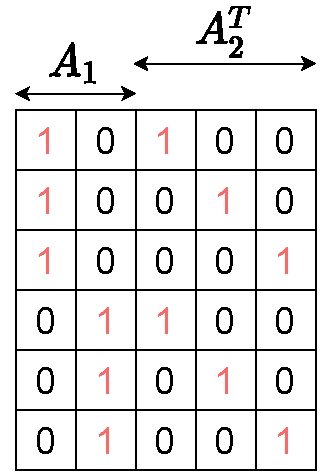
\includegraphics[height=0.25\textheight,keepaspectratio]{./Chapitre2/fig/matrix.pdf}
  \caption{An example of the matrix $A_{12}$ when $n_1=2$ and $n_2=3$.}
  \label{fig:matrix_a12}
\end{figure}

We also have that, the condition $P = P_1 \otimes P_2$ can be rewritten as
$\text{mat}(P) = \vect(P_1) \vect(P_2)^T$. By Lemma 2.1 in \citep{Joel93}, $\text{rank}_+(A) = 1$
if and only if there exist two non-negative vectors $u,v$ such that
$A = u v^T$. Thus, the factorization constraint is equivalent to
$\text{rank}_+\big( \text{mat}(P) \big) = 1$.

\subsection{MMOT-DC}

\subsection{Continuous Co-Optimal Transport} \label{annex:cont_coot}

%%%%%%%%%%%%%%%%%%%%%%%%%%%%%%%%%%%%%%%%%
\begin{proof}[Proof of \Cref{prop:exist_coot}]
  The COOT problem can be rewritten as
  \begin{equation} \label{UCOOT:1}
    \coot(\cX, \cY) = \inf_{\pi \in E_{co}} \int_{\cS} \vert c_X - c_Y \vert^p \; d\pi,
  \end{equation}
  where the set
  \begin{equation}
    E_{co} = \{ \pi \in \cP(\cS): \pi = \pi_1 \otimes \pi_2,
    \text{ where } \pi_k \in U(\mu_k^X, \mu_k^Y) \}.
  \end{equation}
  \Cref{lemma:compact_subset,lemma:coot_continuous}
  below imply that Problem \eqref{UCOOT:1} always admits a minimiser.
\end{proof}
%%%%%%%%%%%%%%%%%%%%%%%%%%%%%%%%%%%%%%%%%%%%%%%%
\begin{lemma} \label{lemma:product_polish}
  Countable product of Polish spaces is also a Polish space.
\end{lemma}
%%%%%%%%%%%%%%%%%%%%%%%%%%%%%%%%%%%%%%%%%
\begin{proof}[Proof of \Cref{lemma:product_polish}]
  First, the countable product of completely metrizable spaces is also completely metrizable
  (see for example, Proposition 1.4 in \citep{Dominique20})

  Second, we show that countable product of seperable spaces is also seperable.
  Given a sequence of seperable spaces $(X_k)_k$,
  let $\mathcal D_k$ be a countable dense subset of $X_k$. For each $k$,
  we fix a point $x_k \in X_k$. For each integer $j \geq 1$, define
  \begin{equation}
    \widetilde{\mathcal D}_j = \prod_{k=1}^j \mathcal D_k \times \prod_{k > j} \{ x_k \}
    \;\; \text{ and } \;\;
    \widetilde{\mathcal D} = \cup_{j} \widetilde{\mathcal D}_j.
  \end{equation}
  Then clearly $\widetilde{\mathcal D}_j$ is countable, for every $j \geq 1$,
  which implies $\widetilde{\mathcal D}$ is also countable.
  To show that $\widetilde{\mathcal D}$ is dense, every neighborhood $\mathcal N$ of
  $(x_1, ..., x_k, ...)$ (after reindexing) is of the form
  $\mathcal N = \prod_{k=1}^j \mathcal O_k \times \prod_{k > j} \{ x_k \}$,
  for some integer $j \geq 1$ and $\mathcal O_k \subset X_k$ is a neighborhood of $x_k$.
  As $\mathcal D_k$ is dense in $X_k$, we have $\mathcal O_k \cap \mathcal D_k \neq \emptyset$,
  thus $\mathcal N \cap \widetilde{\mathcal D} \neq \emptyset$.
  It follows that $\widetilde{\mathcal D}$ is dense in $X$.
  This concludes that the countable product of Polish spaces is also a Polish space.
\end{proof}
%%%%%%%%%%%%%%%%%%%%%%%%%%%%%%%%%%%%%%%%%%%%%%%%
\begin{lemma} \label{lemma:compact_subset}
  If $X_k$ and $Y_k$ are Polish spaces, for every $k = 1, 2$,
  then $E_{co}$ is non-empty and weakly compact in $\cP(\cS)$.
\end{lemma}
%%%%%%%%%%%%%%%%%%%%%%%%%%%%%%%%%%%%%%%%%
\begin{proof}[Proof of \Cref{lemma:compact_subset}]
  Clearly, $(\mu_1^X \otimes \mu_1^Y) \otimes (\mu_2^X \otimes \mu_2^Y) \in E_{co}$,
  so $E_{co}$ is not empty.
  We recall that $U(\mu_1^X, \mu_1^Y, \mu_2^X, \mu_2^Y)$ is the set of admissible couplings
  whose four marginals are $\mu^X_1, \mu^Y_1, \mu^X_2$ and $\mu^Y_2$. First,
  we show that $E_{co} \subset U(\mu_1^X, \mu_1^Y, \mu_2^X, \mu_2^Y)$.
  Indeed, given $\pi_k \in U(\mu_k^X, \mu_k^Y)$, for $k = 1,2$ and denote
  $\pi = \pi_1 \otimes \pi_2 \in E_{co}$. Then, for every $i, k \in \{ 1, 2 \}$ and $i \neq k$,
  we have
  \begin{equation}
      \bigg(\int_{X_{i} \times Y_{i}} d\pi_i \bigg) \int_{Y_k}  d\pi_k = d\mu_k^X.
  \end{equation}
  Other marginal distributions can be calculated in a similar manner and we conclude that
  $\pi \in U(\mu_1^X, \mu_1^Y, \mu_2^X, \mu_2^Y)$.

  As a direct generalization of Lemma 4.4 in \citep{Villani08},
  $U(\mu_1^X, \mu_1^Y, \mu_2^X, \mu_2^Y)$ is weakly compact in $\cP(\cS)$. Thus,
  to show the compactness of $E_{co}$, it is enough to show that $E_{co}$
  is a weakly closed subset of $U(\mu_1^X, \mu_1^Y, \mu_2^X, \mu_2^Y)$.
  Take a sequence $(\pi^{(n)})_n \subset E_{co}$
  such that $\pi^{(n)} \rightharpoonup \pi \in U(\mu_1^X, \mu_1^Y, \mu_2^X, \mu_2^Y)$
  (due to its compactness), we need to show that $\pi \in E_{co}$.
  As $(\pi^{(n)})_n \subset E_{co}$, there exist two sequences
  $(\pi_1^{(n)})_n \subset U(\mu_1^X, \mu_1^Y)$ and $(\pi_2^{(n)})_n \subset U(\mu_2^X, \mu_2^Y)$
  such that $\pi^{(n)} = \pi_1^{(n)} \otimes \pi_2^{(n)}$.

  For each $k = 1, 2$, due to the compactness of $U(\mu_k^X, \mu_k^Y)$ in $\cP(X_k \times Y_k)$
  (Lemma 4.4 in \citep{Villani08}), we can extract a converging subsequence
  $\pi^{(n_i^{(k)})}_k \rightharpoonup \pi_k \in U(\mu_k^X, \mu_k^Y)$, when $i \to \infty$.
  By applying Theorem 2.8 in \citep{Billingsley99} on the Polish space $\cS$
  (thanks to \Cref{lemma:product_polish}), we have
  $\pi^{(n_i^{(1)})}_1 \otimes \pi^{(n_i^{(2)})}_2 \rightharpoonup \pi_1 \otimes \pi_2 \in E_{co}$,
  when $i \to \infty$. This implies $\pi = \pi_1 \otimes \pi_2$, thus $\pi \in E_{co}$.
\end{proof}
%%%%%%%%%%%%%%%%%%%%%%%%%%%%%%%%%
%%%%%%%%%%%%%%%%%%%%%%%%%%%%%%%%%%%%%%%%%%%%%%%%
\begin{lemma} \label{lemma:coot_continuous}
    If $c_X$ and $c_Y$ are bounded measurable functions, then
    the functional $F: \pi \to \Big( \int_{\cS} \vert c_X - c_Y \vert^p \; d\pi \Big)^{1/p}$ is continuous on $E_{co}$.
\end{lemma}
%%%%%%%%%%%%%%%%%%%%%%%%%%%%%%%%%%%%%%%%%
\begin{proof}[Proof of \Cref{lemma:coot_continuous}]
  It is enough to show that $F$ is continuous on $U(\mu_1^X, \mu_1^Y, \mu_2^X, \mu_2^Y)$.
  To do this, we adapt the proof of Lemma 11 in \citep{Chowdhury19} by showing that
  there exists a sequence of continuous functions converging uniformly to $F$.

  As $\cC_b$ is dense in $L^p$ (by applying Proposition 7.9 in \citep{Folland99}
  on Polish spaces endowed with finite measures), there exist two sequences of
  bounded continuous functions $(c_X^{(n)})_n \subset L^p(X, \mu^X)$ and
  $(c_Y^{(n)})_n \subset L^p(Y, \mu^Y)$ such that
  $\vert\vert c_X - c_X^{(n)} \vert\vert_{L^p(X, \mu^X)} \leq 1/n$ and
  $\vert\vert c_Y - c_Y^{(n)} \vert\vert_{L^p(Y, \mu^Y)} \leq 1/n$.

  For each $n \in \bbN$, define $F_n: U(\mu_1^X, \mu_1^Y, \mu_2^X, \mu_2^Y) \to \bbR_{\geq 0}$
  by $F_n(\pi) = \vert\vert c_X^{(n)} - c_Y^{(n)} \vert\vert_{L^p(\cS, \pi)}$.

  The compactness of $U(\mu_1^X, \mu_1^Y, \mu_2^X, \mu_2^Y)$ implies that, for every
  $\pi \in U(\mu_1^X, \mu_1^Y, \mu_2^X, \mu_2^Y)$,
  there exists a sequence $(\pi^{(m)})_m \subset U(\mu_1^X, \mu_1^Y, \mu_2^X, \mu_2^Y)$ such that
  $\pi^{(m)} \rightharpoonup \pi$. In particular, as
  $\vert c_X^{(n)} - c_Y^{(n)} \vert^p \in \cC_b(\cS)$, we have
  \begin{equation}
    \begin{split}
      \lim_{m \to \infty} F_n(\pi^{(m)}) =
      \lim_{m \to \infty} \Big( \int_{\cS} \vert c_X^{(n)} - c_Y^{(n)} \vert^p \;
      d\pi^{(m)} \Big)^{1/p}
      = \Big( \int_{\cS} \vert c_X^{(n)} - c_Y^{(n)} \vert^p \; d\pi \Big)^{1/p} = F_n(\pi).
    \end{split}
  \end{equation}
  We deduce that $F_n$ is sequentially continuous, thus continuous
  (by Remark 5.1.1 in \citep{Ambrosio05}).
  Now, for any $\pi \in U(\mu_1^X, \mu_1^Y, \mu_2^X, \mu_2^Y)$, we have
  \begin{equation}
    \begin{split}
      \vert F_n(\pi) - F(\pi) \vert &=
      \Big\vert \vert\vert c_X^{(n)} - c_Y^{(n)} \vert\vert_{L^p(\cS, \pi)}
      - \vert\vert c_X - c_Y \vert\vert_{L^p(\cS, \pi)} \Big\vert \\
      &\leq \vert\vert c_X^{(n)} - c_Y^{(n)} - (c_X - c_Y) \vert\vert_{L^p(\cS, \pi)} \\
      &\leq \vert\vert c_X^{(n)} - c_X \vert\vert_{L^p(\cS, \pi)} +
      \vert\vert c_Y^{(n)} - c_Y \vert\vert_{L^p(\cS, \pi)} \\
      &= \vert\vert c_X^{(n)} - c_X \vert\vert_{L^p(X, \mu^X)} +
      \vert\vert c_Y^{(n)} - c_Y \vert\vert_{L^p(Y, \mu^Y)} \\
      &\leq 2/n.
    \end{split}
  \end{equation}
  The first inequality follows from a consequence of Minkowski's inequality:
  $ \Big\vert \vert\vert f \vert\vert - \vert\vert g \vert\vert \Big\vert
  \leq \vert\vert f-g \vert\vert$. The second inequality is the Minkowski's inequality.
  This implies that $F_n$ converges uniformly to $F$, thus $F$ is continuous.
\end{proof}
%%%%%%%%%%%%%%%%%%%%%%%%%%%%%%%%%%%%%%%%%%%%%%%%

Before proving the isomorphism and metric properties of COOT, let us first introduce the Monge's
formulation of COOT.
\begin{align}
  \mcoot(\cX, \cY) =
  \inf_{\substack{T_1 \in \cT(\mu^X_1, \mu^Y_1) \\ T_2 \in \cT(\mu^X_2, \mu^Y_2)}}
  \iint \Big|c_X(x_1, x_2) - c_Y \big( T_1(x_1), T_2(x_2) \big) \Big|^p
  \; d\mu^X_1(x_1) \; d\mu^X_2(x_2).
\end{align}
where recall that
$\cT(\mu^X_k, \mu^Y_k) = \{T: X_k \to Y_k \text{ such that } T_{\# \mu^X_k} = \mu^Y_k \}$,
for $k=1,2$. It is not difficult to see that, $\mcoot(\cX, \cY) = 0$ if and only if
$\cX \in \rms(\cY)$. Similar to the GW and Gromo-Monge distances, we have
%%%%%%%%%%%%%%%%%%%%%%%%%%%%%%%
\begin{corollary} \label{coro:coot_mcoot}
  Let $\cX$ and $\cY$ be two measure hypernetworks, then
  \begin{equation}
    \coot(\cX, \cY) = \inf_{\cZ \in \rms(\cX)} \mcoot(\cZ, \cY)
    = \inf_{\cZ \in \rms(\cY)} \mcoot(\cZ, \cX).
  \end{equation}
  Moreover, the infima are always attained: there exist two measure hypernetworks
  $\cZ_x \in \rms(\cX)$ and $\cZ_y \in \rms(\cY)$ such that
  $\coot(\cX, \cY) = \mcoot(\cZ_x, \cY) = \mcoot(\cZ_y, \cX)$.
\end{corollary}
The proof is adapted directly from that of Theorem 14 in \citep{Memoli21}.
For self-contained purpose, we provide the complete proof here.
%%%%%%%%%%%%%%%%%%%%%%%%%%%%%%%%%%%%%%%%%
\begin{proof}[Proof of \Cref{coro:coot_mcoot}]
  Let $(\pi_1^*, \pi_2^*)$ be a solution of the problem $\coot(\cX, \cY)$.
  For $k=1,2$, define the space $Z_k = X_k \times Y_k$
  equipped with the probability measure $\mu_k^Z = \pi_k^* \in U(\mu_k^X, \mu_k^Y)$.
  Define the projection map $P_{X_k}: Z_k \to X_k$ by $P_{X_k}(x,y) = x$ and denote
  $c_Z = (P_{X_1}, P_{X_2})^*c_X$. Clearly, the measure hypernetwork
  $\cZ := ((Z_1, \mu_1^Z), (Z_2, \mu_2^Z), c_Z)$ is a RMS of $\cX$. For
  $k=1,2$, consider the canonical projection map $P_{Y_k}: Z_k \to Y_k$ defined by $P_{Y_k}(x,y) = y$,
  then $P_{Y_k}$ is a transport map from $\mu_k^Z$ to $\mu_k^Y$. Now, as
  $(P_{X_k}, P_{Y_k})_{\#} \mu_k^Z = (P_{X_k}, P_{Y_k})_{\#} \pi_k^* = \pi_k^*$,
  for $k=1,2$, we have
  \begin{align}
    \mcoot(\cZ, \cY) &\leq \int_{Z_1 \times Z_2}
    \big\vert c_Z - (P_{Y_1}, P_{Y_2})^*c_Y \big\vert^p \; d\mu_1^Z \; d\mu_2^Z \\
    &= \int_{Z_1 \times Z_2}
    \big\vert (P_{X_1}, P_{X_2})^*c_X - (P_{Y_1}, P_{Y_2})^*c_Y \big\vert^p
    \; d\mu_1^Z \; d\mu_2^Z \\
    &= \int_{S} \vert c_X - c_Y \vert^p
    \; d(P_{X_1}, P_{Y_1})_{\#} \mu_1^Z \; d(P_{X_2}, P_{Y_2})_{\#} \mu_2^Z \\
    &= \int_{S} \vert c_X - c_Y \vert^p \; d\pi_1^* \; d\pi_2^* \\
    &= \coot(\cX, \cY),
  \end{align}
  and consequently,
  \begin{equation}
    \label{eq:coot_geq_mcoot}
    \coot(\cX, \cY) \geq \inf_{\cZ \in \rms(\cX)} \mcoot(\cZ, \cY).
  \end{equation}
  For the reverse direction, let $\cZ$ be a RMS of $\cX$. Then,
  there exist two transport maps $f_k : Z_k \to X_k$, for $k=1,2$ such that $c_Z = (f_1, f_2)^*c_X$,
  for $\mu_1^Z \otimes \mu_2^Z$-almost everywhere.
  The inequality \eqref{eq:coot_geq_mcoot} implies that we can safely exclude every
  $\cZ \in \rms(\cX)$ with $\mcoot(\cZ, \cY) = \infty$ and consider only those with
  $\mcoot(\cZ, \cY) < \infty$. In this case, there always exists a transport map
  $g_k$ from $\mu_k^Z$ to $\mu_k^Y$, for each $k=1,2$. If we define the map
  $(f_k, g_k): Z_k \to X_k \times Y_k$ by $(f_k,g_k)(z_k) = (f_k(z_k), g_k(z_k))$,
  then $(f_k,g_k)_{\# \mu_k^Z} \in U(\mu_k^X, \mu_k^Y)$, for any $k=1,2$. Now,
  \begin{align}
    \coot(\cX, \cY) &\leq \int_{S} \vert c_X - c_Y \vert^p
    \; d (f_1,g_1)_{\#} \mu_1^Z \; d (f_2,g_2)_{\#} \mu_2^Z \\
    &= \int_{Z_1 \times Z_2} \vert (f_1,f_2)^*c_X - (g_1,g_2)^*c_Y \vert^p \; d\mu_1^Z \; d\mu_2^Z \\
    &= \int_{Z_1 \times Z_2} \vert c_Z - (g_1,g_2)^*c_Y \vert^p \; d\mu_1^Z \; d\mu_2^Z.
  \end{align}
  As this is true for any $\cZ \in \rms(\cX)$ and any corresponding pair of transport maps
  $(g_1, g_2)$, we have
  \begin{equation}
    \coot(\cX, \cY) \leq \inf_{\cZ \in \rms(\cX)} \mcoot(\cZ, \cY).
  \end{equation}
  The equality then follows. Moreover, the first part of the proof also
  shows us how to construct a minimizer $\cZ_x \in \rms(\cX)$ such that
  $\coot(\cX, \cY) = \mcoot(\cZ_x, \cY)$. Similarly, we have
  \begin{equation}
    \coot(\cY, \cX) = \inf_{\cZ \in \rms(\cY)} \mcoot(\cZ, \cX).
  \end{equation}
  By the symmetry of COOT, we deduce that
  \begin{equation}
    \inf_{\cZ \in \rms(\cX)} \mcoot(\cZ, \cY) = \inf_{\cZ \in \rms(\cY)} \mcoot(\cZ, \cX),
  \end{equation}
  and there exists $\cZ_y \in \rms(\cY)$ such that $\coot(\cX, \cY) = \mcoot(\cZ_y, \cX)$.
\end{proof}
%%%%%%%%%%%%%%%%%%%%%%%%%%%%%%%%%%%%%%%%%%%%%%%%

\begin{proof}[Proof of \Cref{prop:coot_iso}]
    Suppose two measure hypernetworks $\cX$ and $\cY$ are weakly isomorphic,
    then there exists a measure hypernetwork $\cZ^*$ which is a common RMS of $\cX$ and $\cY$.
    In particular, $\mcoot(\cZ^*, \cY) = 0$. By \Cref{coro:coot_mcoot}, we deduce that
    \begin{equation}
      \coot(\cX, \cY) = \inf_{\cZ \in \rms(\cX)} \mcoot(\cZ, \cY) = 0.
    \end{equation}
    Now, suppose $\coot(\cX, \cY)=0$, then by \Cref{coro:coot_mcoot},
    there exists a mass splitting $\cZ^*$ of $\cX$ such that
    $\mcoot(\cZ^*, \cY) = 0$. But this also means $\cZ^*$ is a RMS of $\cY$.
    We conclude that $\cX$ and $\cY$ are weakly isomorphic.
\end{proof}
%%%%%%%%%%%%%%%%%%%%%%%%%%%%%%%

%%%%%%%%%%%%%%%%%%%%%%%%%%%%%%%
\begin{proof}[Proof of \Cref{prop:metric_prop}]
    For clarity, given three measure hypernetworks $\cX, \cY$ and $\cZ$,
    we denote $\cS_{xy} = \prod_{k=1}^2 X_k \times Y_k, \cS_{yz} = \prod_{k=1}^2 Y_k \times Z_k,
    \cS_{xz} = \prod_{k=1}^2 X_k \times Z_k$ and $\cS_{xyz} = \prod_{k=1}^2 X_k \times Y_k \times Z_k$.
    \begin{enumerate}
      \item The positiveness is trivial. By \Cref{prop:coot_iso},
      $\coot(\cX, \cY) = 0$ if and only if $\cX$ and $\cY$ are weakly isomorphic.

      \item To show the symmetry, for each $k = 1, 2$, we define the bijection
      $f_k: X_k \times Y_k \to Y_k \times X_k$ by $f_k(x_k,y_k) = (y_k,x_k)$.
      Then, for any $\pi_k \in U(\mu_k^X, \mu_k^Y)$, where $k=1,2$, we have
      $(f_k)_{\#} \pi_k \in U(\mu_k^Y, \mu_k^X)$ and
      \begin{equation}
        \begin{split}
          \coot(\cX, \cY) &= \inf_{\substack{\pi_k \in U(\mu^X_k, \mu^Y_k) \\
          \forall k = 1,2}} \int_{\cS_{xy}} \vert c_X - c_Y \vert^p \; d \pi_1 \; d \pi_2 \\
          &= \inf_{\substack{\pi_k \in U(\mu^X_k, \mu^Y_k) \\
          \forall k = 1,2}} \int_{\cS_{yx}} \vert c_Y - c_X \vert^p \; d (f_1)_{\#} \pi_1 \; d (f_2)_{\#} \pi_2 \\
          &= \inf_{\substack{\gamma_k \in U(\mu^Y_k, \mu^X_k) \\
          \forall k = 1,2}} \int_{\cS_{yx}} \vert c_Y - c_X \vert^p \; d \gamma_1 \; d \gamma_2 \\
          &= \coot(\cY, \cX).
        \end{split}
      \end{equation}

      \item Now, we show the triangle inequality. Let $(\pi^{(YZ)}_1, \pi^{(YZ)}_2)$ and
      $(\pi^{(XZ)}_1, \pi^{(XZ)}_2)$ be the optimal couplings which minimize
      $\coot(\cY, \cZ)$ and $\coot(\cX, \cZ)$, respectively, where
      $\pi^{(YZ)}_k$ and $\pi^{(XZ)}_k$ are in $U(\mu_k^Y, \mu_k^Z)$ and $U(\mu_k^X, \mu_k^Z)$,
      respectively, for every $k=1,2$.

      For each $k = 1,2$, by the glueing lemma (Lemma 7.6 in \citep{Villani03}), there exists a probability measure
      $\sigma_k \in \cP(X_k \times Y_k \times Z_k)$ such that
      $(P_{X_k Y_k})_{\#} \sigma_k = \pi^{(XY)}_k$ and
      $(P_{X_k Y_k})_{\#} \sigma_k = \pi^{(YZ)}_k$. Here, we define the projection maps
      \begin{itemize}
        \item[$\bullet$] $P_{X_k}: X_k \times Y_k \times Z_k \to X_k$, where
        $P_{X_k}(x,y,z) = x$.
        \item[$\bullet$] $P_{X_k Y_k}: X_k \times Y_k \times Z_k \to X_k \times Y_k$,
        where $P_{X_k Y_k}(x,y,z) = (x,y)$.
        \item[$\bullet$] $P_{X_1 Z_1 X_2 Z_2}: \cS_{xyz} \to \cS_{xz}$, where
        $P_{X_1 Z_1 X_2 Z_2}(x_1,y_1,z_1, x_2, y_2, z_2) = (x_1,z_1, x_2, z_2)$.
      \end{itemize}
      and all other projection maps are defined similarly. It follows that
      $(P_{X_k})_{\#} \sigma_k = \mu_k^X$ and $(P_{Z_k})_{\#} \sigma_k = \mu_k^Z$, thus
      $(P_{X_k Z_k})_{\#} \sigma_k \in U(\mu_k^X, \mu_k^Z)$. Furthermore, one also has
      $(P_{X_1 Z_1 X_2 Z_2})_{\#} \sigma =
      (P_{X_1 Z_1})_{\#} \sigma_1 \otimes (P_{X_2 Z_2})_{\#} \sigma_2$,
      where $\sigma = \sigma_1 \otimes \sigma_2$. Indeed, for any function $\phi \in \cC_b(\cS_{xz})$, we have
      \begin{equation}
        \begin{split}
          \int_{\cS_{xz}} \phi \; d(P_{X_1 Z_1 X_2 Z_2})_{\#} \sigma
          &= \int_{\cS_{xyz}} (\phi \circ P_{X_1 Z_1 X_2 Z_2}) \; d\sigma \\
          &= \int_{\cS_{xyz}} (P_{X_1 Z_1}, P_{X_2 Z_2})^*\phi
          \; d \sigma_1 \; d \sigma_2 \\
          &= \int_{\cS_{xz}} \phi \; d (P_{X_1 Z_1})_{\#} \sigma_1 \;
          d (P_{X_2 Z_2})_{\#} \sigma_2.
        \end{split}
      \end{equation}
      Here, with slight abuse of notation, we write $\phi(x_1,y_1, x_2,y_2) = \phi\big( (x_1,y_1), (x_2,y_2) \big)$. Now,
      \begin{equation}
        \begin{split}
          &\coot(\cX, \cZ)^{1/p} \\
          &\leq \Big( \int_{\cS_{xz}} \vert c_X - c_Z \vert^p
          \; d (P_{X_1 Z_1})_{\#} \sigma_1 \; d (P_{X_2 Z_2})_{\#} \sigma_2 \Big)^{1/p} \\
          &= \Big( \int_{\cS_{xz}} \vert c_X - c_Z \vert^p
          \; d(P_{X_1 Z_1 X_2 Z_2})_{\#} \sigma \Big)^{1/p} \\
          &= \Big( \int_{\cS_{xyz}} \big( \vert c_X - c_Z \vert^p \circ P_{X_1 Z_1 X_2 Z_2} \big)
          \; d \sigma \Big)^{1/p} \\
          &\leq \Big( \int_{\cS_{xyz}} \big( \vert c_X - c_Y \vert^p \circ P_{X_1 Y_1 X_2 Y_2} \big)
          \; d \sigma \Big)^{1/p} +
          \Big( \int_{\cS_{xyz}} \big( \vert c_Y - c_Z \vert^p \circ P_{Y_1 Z_1 Y_2 Z_2} \big)
          \; d \sigma \Big)^{1/p} \\
          &= \Big( \int_{\cS_{xy}} \vert c_X - c_Y \vert^p
          \; d (P_{X_1 Y_1 X_2 Y_2})_{\#} \sigma \Big)^{1/p}  +
          \Big( \int_{\cS_{yz}} \vert c_Y - c_Z \vert^p
          \; d (P_{Y_1 Z_1 Y_2 Z_2})_{\#} \sigma \Big)^{1/p}  \\
          &= \Big( \int_{\cS_{xy}} \vert c_X - c_Y \vert^p
          \; d (P_{X_1 Y_1})_{\#} \sigma_1 \; d (P_{X_2 Y_2})_{\#} \sigma_2 \Big)^{1/p} \\
          &+ \Big( \int_{\cS_{yz}} \vert c_Y - c_Z \vert^p
          \; d (P_{Y_1 Z_1})_{\#} \sigma_1 \; d (P_{Y_2 Z_2})_{\#} \sigma_2 \Big)^{1/p} \\
          &= \Big( \int_{\cS_{xy}} \vert c_X - c_Y \vert^p \; d \pi^{(XY)}_1 \; d \pi^{(XY)}_2 \Big)^{1/p}  +
          \Big( \int_{\cS_{yz}} \vert c_Y - c_Z \vert^p \; d \pi^{(YZ)}_1 \; d \pi^{(YZ)}_2 \Big)^{1/p} \\
          &= \coot(\cX, \cY)^{1/p} + \coot(\cY, \cZ)^{1/p}.
        \end{split}
      \end{equation}
      The first inequality is due to the sub-optimality of
      $((P_{X_1 Z_1})_{\#} \sigma_1, (P_{X_2 Z_2})_{\#} \sigma_2)$. The second one is
      the Minkowski inequality and the fact that:
      $|c_X(x_1,x_2) - c_Y(y_1,y_2)| \leq |c_X(x_1,x_2) - c_Z(z_1,z_2)| + |c_Z(z_1,z_2) - c_Y(y_1,y_2)|$,
      or more compactly
      \begin{equation}
        \vert c_X - c_Z \vert \circ P_{X_1 Z_1 X_2 Z_2} \leq
        \vert c_X - c_Y \vert \circ P_{X_1 Y_1 X_2 Y_2} +
        \vert c_Y - c_Z \vert \circ P_{Y_1 Z_1 Y_2 Z_2}.
      \end{equation}
    \end{enumerate}
\end{proof}
%%%%%%%%%%%%%%%%%%%%%%%%%%%%%%%%%

%%%%%%%%%%%%%%%%%%%%%%%%%%%%%%%
\begin{proof}
    This is an adaptation from the proof of quantitative bound between OT and regularized OT
    in \citep{Genevay19}.
    Let $\pi^* \in E_{co}$ be a solution of COOT and denote $\pi_{\Delta}$
    its block approximation at scale $\Delta > 0$.
    Clearly, $\pi_{\Delta} \in E_{co}$. The sub-optimality of $\pi_{\Delta}$ implies
    \begin{equation}
      \begin{split}
        0 &\leq \coot_{\varepsilon}(\cX, \cY) - \coot(\cX, \cY) \\
        &\leq \langle \pi_{\Delta}, \vert c_X - c_Y \vert^p \rangle
        - \langle \pi^*, \vert c_X - c_Y \vert^p \rangle +
        \varepsilon \kl(\pi_{\Delta} \vert \mu_1 \otimes \mu_2).
      \end{split}
    \end{equation}
    Now, using the fact that $\vert x - y \vert \leq \max(x,y)$, for every $x, y \geq 0$,
    and for any $i,j$,
    \begin{equation}
      \sup_{(x_1, x_2) \in Q^{\Delta}_{ij}} c_X(x_1,x_2) \leq
      L^a \sup_{(x_1, x_2) \in Q^{\Delta}_{ij}} \vert\vert x_1 - x_2 \vert\vert^a \leq (L \Delta d_x^{1/p})^a,
    \end{equation}
    we have
    \begin{equation}
      \begin{split}
        \langle \pi_{\Delta}, \vert c_X - c_Y \vert^p \rangle
        - \langle \pi^*, \vert c_X - c_Y \vert^p \rangle
        &\leq \langle \pi_{\Delta}, \vert c_X - c_Y \vert^p \rangle \\
        &\leq \sup_{i,j,k,l} \sup_{\substack{(x_1, x_2) \in Q^{\Delta}_{ij} \\ (y_1,y_2) \in Q^{\Delta}_{kl}}}
        \vert c_X(x_1,x_2) - c_Y(y_1,y_2) \vert^p \\
        &\leq \max\big( \sup_{(x_1, x_2) \in Q^{\Delta}_{ij}} c_X(x_1,x_2)^p,
        \sup_{(y_1, y_2) \in Q^{\Delta}_{kl}} c_Y(y_1,y_2)^p \big) \\
        &\leq \max\big( (\Delta Ld_x^{1/p})^{ap}, (\Delta Ld_y^{1/p})^{ap} \big) \\
        &= (\Delta Ld^{1/p})^{ap}.
      \end{split}
    \end{equation}
    The bound for the entropy term is
    \begin{equation}
      \begin{split}
        H(\pi^{\Delta}) \leq (d_x + d_y) \log(\frac{2D}{\Delta}) \leq 2 d \log(\frac{2D}{\Delta}).
      \end{split}
    \end{equation}
    Thus
    \begin{equation}
      \langle \pi_{\Delta}, \vert c_X - c_Y \vert^p \rangle -
      \langle \pi^*, \vert c_X - c_Y \vert^p \rangle + \varepsilon H(\pi^{\Delta})
      \leq (\Delta Ld^{1/p})^{ap} + 2 d \varepsilon \log(\frac{2D}{\Delta}).
    \end{equation}
    The RHS is a convex function of $\Delta$, thus admits a minimiser
    $\Delta^{ap} = \frac{2d \varepsilon}{ap (Ld^{1/p})^{ap}}$, thus
    \begin{equation}
      \langle \pi_{\Delta}, \vert c_X - c_Y \vert^p \rangle
      - \langle \pi^*, \vert c_X - c_Y \vert^p \rangle + \varepsilon H(\pi^{\Delta})
      \leq \frac{2 d \varepsilon}{ap}
      + \frac{2d \varepsilon}{ap} \log\Big( \frac{ap (2DLd^{1/p})^{ap}}{2d \varepsilon} \Big).
    \end{equation}
\end{proof}
%%%%%%%%%%%%%%%%%%%%%%%%%%%%%%%

%%%%%%%%%%%%%%%%%%%%%%%%%%%%%%
\begin{proof}
    Recall that
    \begin{equation}
      E_{co} = \{ \pi \in \cP(\cS): \pi = \pi_1 \otimes \pi_2,
      \text{ where } \pi_k \in U(\mu_k^X, \mu_k^Y) \}.
    \end{equation}
    First, observe that if $\pi \in E_{co}$ is a solution of COOT, then for any $\gamma \in E_{co}$, one has
    \begin{equation}
      \begin{split}
        0 &\leq \coot_{\varepsilon}(\cX, \cY) - \coot(\cX, \cY) \\
        &\leq \left( \int_{\cS} \vert c_X - c_Y \vert^p \; d\gamma - \int_{\cS} \vert c_X - c_Y \vert^p \; d\pi \right) +
        \varepsilon \kl(\gamma \vert \mu_1 \otimes \mu_2).
      \end{split}
    \end{equation}
    The idea is to choose $\gamma \in E_{co}$ such that, for small $\varepsilon$, the quantity inside the bracket can be arbitrarily small
    (but still positive, due to the optimality of $\pi$), and the KL divergence is always controlled, so that it does not blow up too fast.
    To do so, we extend the block approximation technique in
    \citep{Carlier17} to the multi-marginal case.
    \begin{definition}
      (Block approximation) Given an integer $K \geq 2$ and $p \geq 1$. For each $k=1,...,K$,
      let $\mu_k \in \cP(\bbR^{n_k})$, for some integer $n_k \geq 1$, be a probability measure
      with finite entropy and $p^{\text{th}}$-moment and
      absolutely continuous with respect to the Lebesgue measure.

      For each $a_k = (a_k^{(1)}, ...,a_k^{(n_k)}) \in \cZ^{n_k}$, we define the unit hypercube
      $Q_{a_k} = [a_k^{(1)}, a_k^{(1)} + 1) \times ... \times [a_k^{(n_k)}, a_k^{(n_k)} + 1) \subset \bbR^{n_k}$ and for $\Delta > 0$,
      we denote $Q^{\Delta}_{a_k} = \Delta \cdot Q_{a_k} \subset \bbR^{n_k}$ the rescaled hypercube by $\Delta$ of $Q_{a_k}$.
      For each $\pi \in \cP(\prod_k \bbR^{n_k})$, we define its block approximation at scale $\Delta$ by
      \begin{equation}
        \pi_{\Delta} := \sum_{\substack{a_k \in \cZ^{n_k} \\ k = 1, ..., K}}
        \pi \big(\prod_{k=1}^K Q^{\Delta}_{a_k}\big) \big( \otimes_{k=1}^K \mu_k^{\Delta} \big),
      \end{equation}
      where, for every Borel set $E_k \subset \bbR^{n_k}, \mu_k^{\Delta}$ is the restriction of $\mu_k$ on $Q^{\Delta}_{a_k}$ defined by
      \begin{equation}
        \mu_k^{\Delta}(E_k):=
        \begin{cases}
          \frac{\mu_k(E_k \cap Q^{\Delta}_{a_k})}{\mu_k(Q^{\Delta}_{a_k})} \; ,\text{ if } \mu_k(Q^{\Delta}_{a_k}) > 0 \\
          0 \;\;\;\;\;\;\;\;\;\;\;\;\;\;\;\;,\text{ otherwise}.
        \end{cases}
      \end{equation}
    \end{definition}
    It is not difficult to see that block approximation of a product measure is also a product measure. Indeed, it is enough to consider the case
    $K=2$. Suppose that $\pi = \pi_1 \otimes \pi_2$, then,
    \begin{equation}
      \pi_{\Delta} = \sum_{a_1, a_2}
      \pi_1(Q^{\Delta}_{a_1}) \; \pi_2(Q^{\Delta}_{a_2}) \; \mu_1^{\Delta} \otimes \mu_2^{\Delta} =
      \left( \sum_{a_1} \pi_1(Q^{\Delta}_{a_1}) \; \mu_1^{\Delta} \right) \otimes
      \left( \sum_{a_2} \pi_2(Q^{\Delta}_{a_2}) \; \mu_2^{\Delta} \right).
    \end{equation}
    %%%%%%%%%%%%%%%%%%%%%%%%%%%%%%%%%%%%%%%%%%%%%
    \begin{lemma}
        \label{lemma:block_approx}
      Recall that $U(\mu_1, ..., \mu_K)$ is the set of couplings whose marginals are $\mu_1,...,\mu_K$.
      For each $\pi \in U(\mu_1, ..., \mu_K)$, denote $\pi_{\Delta}$ its block approximation at scale $\Delta > 0$.
      \begin{enumerate}
        \item The entropy $H(\pi)$ is well defined and
        \begin{equation}
          \kl(\pi \vert \otimes_k \mu_k) = H(\pi) - \sum_{k=1}^K H(\mu_k).
        \end{equation}

        \item For every $\Delta > 0, \pi_{\Delta} \in U(\mu_1, ..., \mu_K)$.

        \item Suppose the product space $\prod_k \bbR^{n_k}$ is endowed with the metric
        \begin{equation}
          d((x_1, ..., x_K), (y_1, ..., y_K)) = \Big( \sum_{k=1}^K \vert\vert x_k - y_k \vert\vert^p \Big)^{1/p}.
        \end{equation}
        Then
        \begin{equation}
          W^p_{d^p}(\pi, \pi_{\Delta}) \leq \Big( \sum_{k=1}^K n_k \Big) \Delta^p,
        \end{equation}
        where $W_{d^p}(\pi, \pi_{\Delta})$ is the $p$-Wasserstein distance between $\pi$ and $\pi_{\Delta}$ induced by the cost $d^p$.
        Consequently, $\pi_{\Delta} \rightharpoonup \pi$ when $\Delta \to 0$.

        \item There exists constants $C > 0$ and $\alpha \in (0,1)$ such that
        \begin{equation}
          \kl(\pi_{\Delta} \vert \otimes_k \mu_k) \leq
          \sum_{k=1}^K \Big( C \big( M(\mu_k) + n_k \Delta^2 + 1 \big)^{\alpha} - n_k \log \Delta \Big).
        \end{equation}
      \end{enumerate}
    \end{lemma}
    %%%%%%%%%%%%%%%%%%%%%%%%%%%%%%%%%%%%%%%%%
    \begin{proof}
      Most proofs follow directly from \citep{Carlier17}.
      \begin{enumerate}
        \item If $\pi \ll \otimes_k \mu_k$, then as $\mu_k \ll \lambda_k$, we must have $\pi \ll \otimes_k \lambda_k$. Thus $H(\pi)$ is well
        defined. Furthermore,
        \begin{equation}
          \begin{split}
            \kl(\pi \vert \otimes_k \mu_k)
            &= \int \log \Big( \frac{\pi(x_1,...,x_K)}{\mu_1(x_1)...\mu_K(x_K)} \Big) \pi(x_1, ..., x_K) \; dx_1 ... dx_K \\
            &= \int \pi \log \pi - \sum_{k=1}^K \int \pi(x_1, ..., x_K) \log \mu_k(x_k) \; dx_1 ... dx_K \\
            &= H(\pi) - \sum_{k=1}^K \int \pi_{\# k}(x_k) \log \mu_k(x_k) \; dx_k \\
            &= H(\pi) - \sum_{k=1}^K \int \mu_k(x_k) \log \mu_k(x_k) \; dx_k \\
            &= H(\pi) - \sum_{k=1}^K H(\mu_k).
          \end{split}
        \end{equation}

        \item See Proposition 2.10 in \citep{Carlier17}
        \item See Lemma 2.11 and corollary 2.12 in \citep{Carlier17}
        \item See Proposition 2.14 in \citep{Carlier17}.
      \end{enumerate}
    \end{proof}
    %%%%%%%%%%%%%%%%%%%%%%%%%%%%%%%%%%%%%%%%%%%%%
    \begin{lemma} \label{lemma:limsupinf}
      Under Assumption 2a in the Proposition ,
      let $E$ be a non-empty subset of $\cP(\cS)$ and $(\varepsilon_n)_n$ be a positive sequence converging to zero.
      Define $\widetilde{F}: \cP(\cS) \to \bbR \cup \{ \infty \}$ and
      $\widetilde{F}_n: \cP(\cS) \to \bbR \cup \{ \infty \}$ by
      \begin{equation}
        \widetilde{F}(\pi) =
        \begin{cases}
          \int_{\cS} \vert c_X - c_Y \vert^p \; d\pi, \text{ if } \pi \in E \\
          \infty \;\;\;\;\;\;\;\;\;\;\;\;\;\;\;\;\;\;\;\;\; ,\text{ otherwise},
        \end{cases}
      \end{equation}
      and
      \begin{equation}
        \widetilde{F}_n(\pi) =
        \begin{cases}
          \int_{\cS} \vert c_X - c_Y \vert^p \; d\pi + \varepsilon_n \kl(\pi \vert \mu_1 \otimes \mu_2), \text{ if } \pi \in E \\
          \infty \;\;\;\;\;\;\;\;\;\;\;\;\;\;\;\;\;\;\;\;\;\;\;\;\;\;\;\;\;\;\;\;\;\;\;\;\;\;\;\;\;\;\;\;\;\;\;\;\;\;\;\; ,\text{ otherwise}.
        \end{cases}
      \end{equation}
      \begin{enumerate}
        \item Assume that if $\pi \in E$, then so is its block approximation. Then for every $\pi \in E$ and positive sequence $(\Delta_n)_n \to 0$, we have
        \begin{equation}
          \widetilde{F}(\pi) \geq \lim\sup_{n \to \infty} \widetilde{F}_{\Delta_n}(\pi_{\Delta_n}).
        \end{equation}

        \item Let $(\pi_n)_n \subset \cP(\cS)$ be a sequence weakly converging to $\pi \in E$. Then
        \begin{equation}
          F(\pi) \leq \lim \inf_{n \to \infty} F_{n}(\pi_n).
        \end{equation}
      \end{enumerate}
    \end{lemma}
    %%%%%%%%%%%%%%%%%%%%%%%%%%%%%%%%%%%%%%%%%
    \begin{proof}
      \text{ }
      \begin{enumerate}
        \item When $\cS$ is a finite-dimensional vector space, by \Cref{lemma:block_approx} and
        definition 6.8 in \citep{Villani08}, when $n \to \infty$,
        \begin{equation}
          \int_S \vert c_X - c_Y\vert^p \; d\pi_{\Delta_n} \to \int_S \vert c_X - c_Y\vert^p \; d\pi.
        \end{equation}
        On the other hand, following \Cref{lemma:block_approx} and the proof of the proposition 2.16 in \citep{Carlier17}, we have
        \begin{equation}
          \lim\sup_{n \to \infty} \Delta_n \kl(\pi_{\Delta_n} \vert \mu_1 \otimes \mu_2) \leq 0.
        \end{equation}
        The claim then follows.

        \item This is true because the KL divergence is nonnegative and the other terms are lower semicontinuous.
      \end{enumerate}
    \end{proof}
    %%%%%%%%%%%%%%%%%%%%%%%%%%%%%%%%%%%%%%%%%%%%%
    Now, we complete the proof of the .
    When $\varepsilon \to 0$, in case of finite-dimensional spaces, if $\pi \in E_{co}$ (or $E_{gw}$), then so is its block approximation.
    We deduce from \Cref{lemma:limsupinf} that $\widetilde{F}_{n}$ $\Gamma$-converges to
    $\widetilde{F}$, whenever $E = E_{co}$ or $E = E_{gw}$. Moreover, in both cases, the weak compactness of $E$ implies the equi-coercivity
    of $\widetilde{F}_n$. By the theorems 7.8 and 7.18 in \citep{Maso93}, we deduce that
    $\coot_{\varepsilon_n}(\cX, \cY) \to \coot(\cX, \cY)$, when $\varepsilon_n \to 0$,
    and if $(\pi_{\varepsilon_n})_{n}$ is a sequence of solution of $\coot_{\varepsilon_n}(\cX, \cY)$,
    then any cluster point of $(\pi_{\varepsilon_n})_{n}$ is a solution of $\coot(\cX, \cY)$.
  \end{proof}
%%%%%%%%%%%%%%%%%%%%%%%%%%%%%%%

%%%%%%%%%%%%%%%%%%%%%%%%%%%%%%%%%%%
\section{Proofs in Chapter 3}

For later convenience, we define the function
$\vert \xi_1 - \xi_2 \vert^p: (X_1^s \times X_2^s) \times (X_1^f \times X_2^f) \to \bbR_{\geq 0}$ by
\begin{equation}
    \vert \xi_1 - \xi_2 \vert^p \big((x_1^s, x_2^s), (x_1^f, x_2^f)\big) :=
    \vert \xi_1(x_1^s, x_1^f) - \xi_2(x_2^s, x_2^f) \vert^p,
\end{equation}
and write the objective function of generalized COOT as
\begin{equation}
    F_{\lambda}(\pi^s, \pi^f) = \iint |\xi_1 - \xi_2|^p \mathrm d\pi^s \mathrm d \pi^f
    + \sum_{k=1}^2\lambda_k D_k(\pi^s_{\#k} \otimes \pi^f_{\#k} \vert \mu^s_k \otimes \mu^f_k).
\end{equation}
The generalized COOT now reads compactly as
\begin{equation} \label{eq:ucoot_copy}
%   \ucoot_{\lambda}(\cX_1, \cX_2) :=
  \inf_{\substack{\pi^s \in \cM^+(X_1^s \times X_2^s) \\
  \pi^f \in \cM^+(X_1^f \times X_2^f) \\ m(\pi^s) = m(\pi^f)}} F_{\lambda}(\pi^s, \pi^f)
\end{equation}

%%%%%%%%%%%%%%%%%%%%%%%%%%%%%%%%%%%%%%%%%%
\subsection{Proofs related to the properties of UCOOT}
%%%%%%%%%%%%%%%%%%%%%%%%%%%%%%%%%%%%%%%

%%%%%%%%%%%%%%%%%%%%%%%%%%%%%%%%%%%%%%%%%%
\begin{claim}
  When $D_k = \iota_{=}$ and $\mu_k^s, \mu_k^f$ are probability measures, for $k=1,2$,
  then we recover COOT from generalized COOT.
\end{claim}
%%%%%%%%%%%%%%%%%%%%%%%%%%%%%%%%%%%%%%%%%%
\begin{proof}
  Under the above assumptions, the generalized COOT problem becomes
  \begin{equation}
    \begin{split}
      \inf_{\substack{\pi^s \in \cM^+(X_1^s \times X_2^s) \\
      \pi^f \in \cM^+(X_1^f \times X_2^f)}}
      &\iint |\xi_1 - \xi_2|^p \mathrm d\pi^s \mathrm d \pi^f \\
      \text{subject to } &\pi^s_{\#1} \otimes \pi^f_{\#1} = \mu_1^s \otimes \mu_1^f \text{ (C1) } \\
      & \pi^s_{\#2} \otimes \pi^f_{\#2} = \mu_2^s \otimes \mu_2^f \text{ (C2) } \\
      & m(\pi^s) = m(\pi^f) \text{ (C3) }.
    \end{split}
  \end{equation}
  As $m(\pi) = m(\pi_{\#1}) = m(\pi_{\#2})$,
  for any measure $\pi$, and $\mu_k^s, \mu_k^f$ are probability measures, for $k=1,2$,
  one has $m(\pi^s) m(\pi^f) = 1$, thus $m(\pi^s) = m(\pi^f) = 1$.
  Now, the constraint C1 implies that
  $\int_{X_1^s} \mathrm d\pi^s_{\#1} \mathrm d \pi^f_{\#1}
  = \int_{X_1^s} \mathrm d\mu_1^s \mathrm d\mu_1^f$. Thus, $\pi^f_{\#1} = \mu_1^f$.
  Similarly, we have $\pi^s_{\#k} = \mu_k^s$ and $\pi^f_{\#k} = \mu_k^f$, for any $k=1,2$.
  We conclude that $\pi^f \in U(\mu_1^f, \mu_2^f)$ and $\pi^s \in U(\mu_1^s, \mu_2^s)$,
  and we obtain the COOT problem.
\end{proof}
%%%%%%%%%%%%%%%%%%%%%%%%%%%%%%%%%%%%%%%%%%

%%%%%%%%%%%%%%%%%%%%%%%%%%%%%%%%%%%%%%%%%%
\begin{proposition}
    \label{eq:ucoot_existence_copy}
  (Existence of minimizer) Denote
  $\cS := (X_1^s \times X_2^s) \times (X_1^f \times X_2^f)$.
  Problem \eqref{eq:ucoot_copy} admits a minimizer if at least one of
  the following conditions hold:
  \begin{enumerate}
    \item The entropy functions $\phi_1$ and $\phi_2$ are superlinear, \textit{i.e}.
    $(\phi_1)'_{\infty} = (\phi_2)'_{\infty} = \infty$.
    \item The function $\vert c_X - c_Y \vert^p$ has compact sublevels in $\cS$ and
    $\inf_{\cS} \vert \xi_1 - \xi_2 \vert^p + \lambda_1 (\phi_1)'_{\infty} + \lambda_2 (\phi_2)'_{\infty} > 0$.
  \end{enumerate}
\end{proposition}
%%%%%%%%%%%%%%%%%%%%%%%%%%%%%%%%%%%%%%%%%%

%%%%%%%%%%%%%%%%%%%%%%%%%%%%%%%%%%%%%%%%%%
\begin{proof}
  We adapt the proof of Theorem 3.3 in \citep{Liero18} and of Proposition 3 in \citep{Sejourne20}.
  For convenience, we write $\mu_1 = \mu_1^s \otimes \mu_1^f$ and
  $\mu_2 = \mu_2^s \otimes \mu_2^f$. For each pair $(\pi^s, \pi^f)$, denote
  $\pi = \pi^s \otimes \pi^f$.
  It can be shown that
  $\pi_{\# k} := (P_{X_k^s \times X_k^f})_{\#} \pi
  = (P_{X_k^s})_{\#} \pi^s \otimes (P_{X_k^f})_{\#} \pi^f =
  \pi^s_{\# k} \otimes \pi^f_{\# k}$, for $k=1,2$. Indeed, for any function
  $\phi \in \mathcal C_b(X_k^s \times X_k^f)$, we have
    \begin{equation}
      \begin{split}
        \int_{X_k^s \times X_k^f} \phi \;
        \mathrm d (P_{X_k^s X_k^f})_{\#} \pi
        &= \int_{\cS} (\phi \circ P_{X_k^s X_k^f}) \; \mathrm d\pi \\
        &= \int_{\cS} \phi(x_k^s, x_k^f)
        \; \mathrm d \pi^s(x_1^s, x_2^s) \; \mathrm d \pi^f(x_1^f, x_2^f) \\
        &= \int_{X_k^s \times X_k^f} \phi \; \mathrm d \pi^s_{\# k} \;
        \mathrm d \pi^f_{\# k}.
      \end{split}
    \end{equation}
  Thus, Problem \eqref{eq:ucoot_copy} can be rewritten as
  \begin{equation}
    \ucoot_{\lambda}(\cX_1, \cX_2) =
    \inf_{\pi \in E_{uco}} \int_{\cS} \vert \xi_1 - \xi_2 \vert^p
    \mathrm d\pi + \sum_{k=1,2} \lambda_k D_{\phi_k}(\pi_{\# k} \vert \mu_k),
  \end{equation}
  where
  \begin{equation}
    E_{uco} = \{ \pi \in \cM^+(\cS) \vert \pi = \pi^s \otimes \pi^f,
    \pi^s \in \cM^+(X_1^s \times X_2^s),
    \pi^f \in \cM^+(X_1^f \times X_2^f) \}.
  \end{equation}
  Define
  \begin{equation}
    L(\pi):= \int_{\cS} \vert \xi_1 - \xi_2 \vert^p \mathrm d \pi +
    \sum_{k=1,2} \lambda_k D_{\phi_k}(\pi_{\# k} \vert \mu_k).
  \end{equation}
  By Jensen's inequality, we have
  \begin{equation}
    \begin{split}
      L(\pi) &\geq m(\pi) \inf_{\cS} \vert \xi_1 - \xi_2 \vert^p +
      \sum_{k=1,2} \lambda_k m(\mu_k) \phi_k \Big( \frac{m(\pi_{\# k})}{m(\mu_k)} \Big) \\
      &= m(\pi) \bigg[ \inf_{\cS} \vert \xi_1 - \xi_2 \vert^p +
      \sum_{k=1,2} \lambda_k \frac{m(\mu_k)}{m(\pi)} \phi_k
      \Big( \frac{m(\pi)}{m(\mu_k)} \Big) \bigg],
    \end{split}
  \end{equation}
  where, in the last equality, we use the relation $m(\pi) = m(\pi_{\# k})$, for $k=1,2$.
  It follows from the assumption that $L$ is coercive. So, $L(\pi) \to \infty$
  when $m(\pi) \to \infty$.

  Clearly $\inf_{E_{uco}} L < \infty$ because
  $L\big( (\mu_1^s \otimes \mu_2^s) \otimes (\mu_1^f \otimes \mu_2^f) \big) < \infty$.
  Let $(\pi_n)_n \subset {E_{uco}}$ be a minimizing sequence, meaning that
  $L(\pi_n) \to \inf_{E_{uco}} L$.
  Such sequence is necessarily bounded (otherwise, there exists a subsequence $(\pi_{n_k})_{n_k}$
  with $m(\pi_{n_k}) \to \infty$ and the coercivity of $L$ implies $L(\pi_{n_k}) \to \infty$,
  which is absurd). Suppose $m(\pi_{n}) \leq M$, for some $M > 0$. By Tychonoff's theorem,
  as $X_k^s$ and $X_k^f$ are compact spaces,
  so is the product space $\cS$. Thus, by Banach-Alaoglu theorem,
  the ball $B_M = \{ \pi \in \cM^+(\cS): m(\pi) \leq M \}$
  is weakly compact in $\cM^+(\cS)$.

  Consider the set $\overline{E}_{uco} = E_{uco} \cap B_M$, then clearly
  $(\pi_n)_n \subset \overline{E}_{uco}$. We will show that
  there exists a converging subsequence of $(\pi_n)_n$, whose limit is in $\overline{E}_{uco}$,
  thus $\overline{E}_{uco}$ is weakly compact. Indeed, by definition of $E_{uco}$,
  there exist two sequences $(\pi_n^s)_n$ and $(\pi_n^f)_n$ such that
  $\pi_n = \pi_n^s \otimes \pi_n^f$.
  We can assume furthermore that $m(\pi_n^s) = m(\pi_n^f) = \sqrt{m(\pi_n)} \leq \sqrt M$.
  As $m(\pi_n^s)$ and $m(\pi_n^f)$ are bounded, by reapplying Banach-Alaoglu theorem,
  one can extract two converging subsequences (after reindexing)
  $\pi_n^s \rightharpoonup \pi^s \in \cM^+(X_1^s \times X_2^s)$ and
  $\pi_n^f \rightharpoonup \pi^f \in \cM^+(X_1^f \times X_2^f)$,
  with $m(\pi^s) = m(\pi^f) \leq \sqrt{M}$.
  An immediate extension of Theorem 2.8 in \citep{Billingsley99} to the convergence of
  the products of bounded positive measures implies
  $\pi_n^s \otimes \pi_n^f \rightharpoonup \pi^s \otimes \pi^f \in \overline{E}_{uco}$.

  Now, the lower semicontinuity of $L$ implies that $\inf_{E_{uco}} L \geq L(\pi^s \otimes \pi^f)$,
  thus $L(\pi^s \otimes \pi^f) = \inf_{E_{uco}} L$ and $(\pi^s, \pi^f)$
  is a solution of Problem \eqref{eq:ucoot_copy}.
\end{proof}
%%%%%%%%%%%%%%%%%%%%%%%%%%%%%%%%%%%%%%%%%%%%%

%%%%%%%%%%%%%%%%%%%%%%%%%%%%%%%%%%%%%%%%%%%
\begin{claim}
  Suppose that $\cX_1$ and $\cX_2$ are two finite sample-feature spaces such that
  $(X^s_1, X^s_2)$ and $(X^f_1, X^f_2)$
  have the same cardinality and are equipped with the uniform measures
  $\mu_1^s = \mu_2^s$, $\mu_1^f = \mu_2^f$. Then $\ucoot_{\lambda}(\cX_1, \cX_2) = 0$
  if and only if there exist perfect alignments between rows (samples) and between
  columns (features) of the interaction matrices $\xi_1$ and $\xi_2$.
\end{claim}
%%%%%%%%%%%%%%%%%%%%%%%%%%%%%%%%%%%%%%%%%%%%%
\begin{proof}
  Without loss of generality, we can assume that $\mu_k^s$ and $\mu_k^f$ are
  discrete uniform probability distributions, for $k=1,2$. By Proposition 1 in \citep{Redko20},
  under the assumptions on $\cX_1$ and $\cX_2$, we have
  $\coot(\cX_1, \cX_2) = 0$ if and only if there exist perfect alignments
  between rows (samples) and between columns (features) of the interaction matrices $\xi_1$ and
  $\xi_2$. So, it is enough to prove that $\ucoot_{\lambda}(\cX_1, \cX_2) = 0$
  if and only if $\coot(\cX_1, \cX_2) = 0$.

  Let $(\pi^s, \pi^f)$ be a pair of equal-mass couplings such that
  $\ucoot_{\lambda}(\cX_1, \cX_2) = 0$. It follows that
  $\pi^s_{\#k} \otimes \pi^f_{\#k} = \mu_k^s \otimes \mu_k^f$, for $k=1,2$. Consequently,
  $m(\pi^s) m(\pi^f) = m(\mu_1^s) m(\mu_1^f) = 1$, so $m(\pi^s) = m(\pi^f) = 1$. Now, we have
  $\int_{X_k^s} \mathrm d \pi^s_{\#k} \; \mathrm d \pi^f_{\#k}
  = \int_{X_k^s} \mathrm d\mu_k^s \; \mathrm d\mu_k^f$, or equivalently,
  $\pi^f_{\#k} = \mu_k^f$. Similarly, $\pi^s_{\#k} = \mu_k^s$, meaning that
  $\pi^s \in U(\mu_1^s, \mu_2^s)$ and $\pi^f \in U(\mu_1^f, \mu_2^f)$. Thus,
  $\coot(\cX_1, \cX_2) = \ucoot_{\lambda}(\cX_1, \cX_2) = 0$.

  For the other direction, suppose that $\coot(\cX_1, \cX_2) = 0$.
  Let $(\pi^s, \pi^f)$ be a pair of couplings such that $\coot(\cX_1, \cX_2) = 0$.
  As $\pi^s \in U(\mu_1^s, \mu_2^s)$ and $\pi^f \in U(\mu_1^f, \mu_2^f)$, one has
  $\coot(\cX_1, \cX_2) = F_{\lambda}(\pi^s, \pi^f) \geq
  \ucoot_{\lambda}(\cX_1, \cX_2) \geq 0$,
  for every $\lambda_1, \lambda_2 > 0$. So, $\ucoot_{\lambda}(\cX_1, \cX_2) = 0$.
\end{proof}
%%%%%%%%%%%%%%%%%%%%%%%%%%%%%%%%%%%

%%%%%%%%%%%%%%%%%%%%%%%%%%%%%%%%%%%ù
\subsection{Robustness of UCOOT and sensitivity of COOT}

First, we recall our assumptions.
%%%%%%%%%%%%%%%%%%%%%%%%%%%%%%%%%%%%%%%%%
\begin{assumption}
\label{assump:robust_copy}
Consider two sample-feature spaces
$\bbX_k = ((X^s_k, \mu^s_k), (X^f_k, \mu^f_k), \xi_k)$, for $k=1,2$.
Let $\varepsilon^s$ (resp. $\varepsilon^f$) be a probability measure with compact support $O^s$
(resp. $O^f$). For $a \in \{s, f\}$, define the noisy distribution
$\widetilde{\mu}^a = \alpha_a \mu^a + (1-\alpha_a) \varepsilon^a$, where $\alpha_a \in [0,1]$.
We assume that $\xi_1$ is defined on
$(X^s_1 \cup O^s) \times (X^f_1 \cup O^f)$ and that $\xi_1, \xi_2$
are continuous on their supports. We denote the contaminated sample-feature space by
$\widetilde{\cX_1} = ((X^s_1 \cup O^s, \widetilde{\mu}^s_1),
(\cX^f_1 \cup O^f, \widetilde{\mu}^f_1), \xi_1)$. Finally,
we define some useful minimal and maximal costs:
  \[
  \begin{cases}
  \Delta_{0} =& \min_{
  \substack{
       x_1^s \in O^s, x_1^f \in O^f  \\
       x_2^s \in \cX_2^s, x_2^f \in \cX_2^f
  }}\quad |\xi_1(x_1^s, x_1^f) - \xi_2(x_2^s, x_2^f)|^p \\
  \Delta_{\infty} =& \max_{
  \substack{
  x_1^s \in \cX_1^s \cup O^s, x_1^f \in \cX_1^f \cup O^f \\
  x_2^s \in \cX_2^s, x_2^f \in \cX_2^f
  }} \quad|\xi_1(x_1^s, x_1^f) - \xi_2(x_2^s, x_2^f)|^p \enspace.
  \end{cases}
\]
\end{assumption}
For convenience, we write $C = \vert \xi_1 - \xi_2 \vert^p$ and
$\widetilde{\cS} := (X^s_1 \cup O^s) \times X_2^s \times (X^f_1 \cup O^f) \times X_2^f$.
%%%%%%%%%%%%%%%%%%%%%%%%%%%%%%%%
\begin{proposition}[COOT is sensitive to outliers]
Consider $\widetilde{\cX_1}, \cX_2$ as defined in \Cref{assump:robust_copy}.
Then:
 \label{prop:coot-not-robust_copy}
\begin{equation}
    \coot(\widetilde{\cX_1}, \cX_2) \geq (1 - \alpha_s)(1-\alpha_f) \Delta_0.
\end{equation}
%%%%%%%%%%%%%%%%%%%%%%%%%%%%%%%%%
\end{proposition}
\begin{proof}
Consider a pair of feasible alignments $(\pi^s, \pi^f)$. Since $C$ is non-negative, taking the COOT integral over a smaller set leads to the lower bound:
% \coot(\cX_1, \widetilde{\cX_2}) &= \min_{\substack{\pi^s \in \cU(\mu_1^s, \widetilde{\mu_2^s}) \\ \pi^f \in \cU(\mu_1^f, \widetilde{\mu_2^f})}}
\begin{equation}
    \begin{split}
        \int_{\widetilde{\cS}} C \mathrm d\pi^s\mathrm d\pi^f
        &\geq \int_{O^s \times \cX_2^s \times O^f \times \cX_2^f} C \mathrm d\pi^s\mathrm d\pi^f \\
          &\geq  \Delta_0 \int_{O^s \times \cX_2^s \times O^f \times \cX_2^f}  \mathrm d\pi^s\mathrm d\pi^f \\
          &= \Delta_0 \int_{O^s\times O^f}  \mathrm d\pi^s_{\#1} \mathrm d\pi^f_{\#1} \\
          &\geq (1 - \alpha_s)(1 -\alpha_f)\Delta_0,
    \end{split}
\end{equation}
where the last inequality follows from the marginal constraints.
\end{proof}

%%%%%%%%%%%%%%%%%%%%%%%%%%%%%%%%%
\begin{theorem}[UCOOT is robust to outliers]
  \label{thm:ucoot_robust_copy}
  Consider two sample-feature spaces $\widetilde{\cX_1}, \cX_2$ as defined in
  \Cref{assump:robust_copy}. Let
  $\delta = 2(\lambda_1 + \lambda_2)(1 - \alpha_s\alpha_f)$ and
  $K = M + \frac{1}{M}\ucoot(\cX_1, \cX_2) +\delta$, where
  $M= m(\pi^s) = m(\pi^f)$ is the transported mass between clean data. Then:
     \begin{equation} %\label{eq:ucoot-robust}
      \begin{split}
        \ucoot(\widetilde{\cX_1}, \cX_2)
        \leq \alpha_s \alpha_f \ucoot(\cX_1, \cX_2) +
        \delta M \left[ 1 - \exp \left( {- \frac{\Delta_{\infty}(1+M) + K}{\delta M}} \right) \right].
      \end{split}\vspace{-10mm}
    \end{equation}
  \end{theorem}
  %%%%%%%%%%%%%%%%%%%%%%%%%%%%%%%%%%%%%%%%%%%%
  To get the exponential bound of this theorem, we use the following lemma.
  \begin{lemma}
  \label{slem:bound}
  Let $\varphi: t \in (0, 1] \mapsto t\log(t) - t + 1$ and
  $f_{a, b}: t \in (0, 1] \mapsto t \to at + b \varphi(t)$ for some $a, b > 0$.
  Then:
  \begin{equation}
      \min_{t \in (0, 1]} f_{a, b}(t) = b(1 - e^{-a/b}) = f_{a, b}(e^{-\frac{a}{b}}).
  \end{equation}
  \end{lemma}
  \begin{proof}
    Since $f_{a,b}$ is convex, cancelling the gradient is sufficient for optimality.
    The solution follows immediately.
  \end{proof}
  \begin{proof}
    The proof uses the same core idea of \citep{Fatras21} but is slightly more technical
    for two reasons: (1) we consider arbitrary outlier distributions instead of simple Diracs;
    (2) we consider sample-feature outliers which requires more technical derivations.

    The idea of proof is as follows. First, we construct sample and feature couplings
    from the solution of "clean" UCOOT and the reference measures. Then, they are used to
    upper bound the "noisy" UCOOT. By manipulating this bound, the "clean" UCOOT term will appear.
    A variable $t \in (0,1)$ is also introduced in the fabricated couplings.
    The upper bound becomes a function of $t$ and can be optimized to obtain the final bound.

    Now, we prove Theorem 2.

    \paragraph{Fabricating sample and feature couplings.}
    Given the equal-mass solution $(\pi^s, \pi^f)$ of the UCOOT problem,
    with $m(\pi^s) = m(\pi^f) = M$, consider, for $t \in (0,1)$, a pair of
    sub-optimal transport plans:
    \begin{align}
      &\widetilde{\pi}^s = \alpha_s \pi^s + t (1-\alpha_s) \varepsilon_s \otimes \mu^s_2\\
      &\widetilde{\pi}^f = \alpha_f \pi^f + t (1-\alpha_f) \varepsilon_f \otimes \mu^f_2.
    \end{align}
    Then, for $a\in \{s, f\}$, it holds:
    \begin{itemize}
      \item $\widetilde{\pi}^a_{\#1} = \alpha_k \pi^a_{\#1} + t (1 - \alpha_a) \varepsilon_a$,
      \item $\widetilde{\pi}^a_{\#2} = \alpha_k \pi^a_{\#2} + t (1 - \alpha_a) \mu^a_2$,
      \item $m(\widetilde{\mu}^a_1) = 1$ and $m(\widetilde{\pi}^a) = \alpha_a M + (1-\alpha_a) t$.
    \end{itemize}
    \paragraph{Establishing and manipulating the upper bound.}
    Denote $q = (1 - \alpha_s)(1 - \alpha_f), s = \alpha_s (1-\alpha_f) + \alpha_f (1 - \alpha_s)$
    and recall that on $\widetilde{\cS}$, the cost $C$ is upper bounded by
    $\Delta_{\infty} = \max_{\widetilde{\cS}}|\xi_1 - \xi_2|^p$.
    First we upper bound the transportation cost:
    \begin{equation}
      \label{seq:cost-split}
      \begin{split}
        &\int_{\widetilde{\cS}} C \; \mathrm d\widetilde{\pi}^s \; \mathrm d\widetilde{\pi}^f \\
        &= \alpha_s\alpha_f\int_{\widetilde{\cS}} C \; \mathrm d\pi^s \; d\pi^f +
        t \sum_{k \neq i} (1-\alpha_i) \alpha_k \int_{\widetilde{\cS}} C \;
        \mathrm d \varepsilon_i \; \mathrm d\mu^i_2  \; \mathrm d\pi^k +
        q t^2 \int_{\widetilde{\cS}} C \; \mathrm d \varepsilon_s \; \mathrm d\mu_2^s \;
        \mathrm d\varepsilon_f \; \mathrm d\mu^f_2 \\
        &\leq \alpha_s\alpha_f \int_{\cS} C \; \mathrm d\pi^s \;\mathrm d\pi^f +
        \Delta_{\infty}(Ms + q)t\enspace,
      \end{split}
    \end{equation}
   since $t^2 \leq t$.

  Second, we turn to the KL marginal discrepancies. We would like to extract the KL terms
  involving only the clean transport plans from the contaminated ones.
  We first detail both joint KL divergences for the source measure indexed by 1.
  The same holds for the target measure:
    \begin{equation}
    \label{seq:kl-split}
    \begin{split}
      &\kl(\widetilde{\pi}^s_{\#1} \otimes \widetilde{\pi}^f_{\#1} \vert \widetilde{\mu}^s_1 \otimes \widetilde{\mu}^f_1) =
      \sum_{k \neq i} m(\widetilde{\pi}^i) \kl(\widetilde{\pi}^k_{\#1} \vert \widetilde{\mu}^k_1) +
      \prod_{k} \big( m(\widetilde{\pi}^k) - 1 \big)\\
      &
      \kl(\pi^s_{\#1} \otimes \pi^f_{\#1} \vert \mu^s_1 \otimes \mu^f_1) =
    M \sum_k \kl(\pi^k_{\#1} \vert \mu^k_1) + (M-1)^2.
      \end{split}
    \end{equation}
    Now we upper bound each smaller KL term using the joint convexity of the KL divergence:
    \begin{equation}
      \begin{split}
        \kl(\widetilde{\pi}^k_{\#1} \vert \widetilde{\mu}^k_1) &\leq
        \alpha_k \kl(\pi^k_{\#1} \vert \mu^k_1) + (1 - \alpha_k) \kl(t \varepsilon_k \vert \varepsilon_k) \\
        &= \alpha_k \kl(\pi^k_{\#1} \vert \mu^k_1) + (1 - \alpha_k) \varphi(t),
      \end{split}
    \end{equation}
    where $\varphi(t) = t \log t - t + 1$, for $t > 0$. Thus, for $k\neq i$:
    \begin{equation}
      \begin{split}
        &m(\widetilde{\pi}^i) \kl(\widetilde{\pi}^k_{\#1} \vert \widetilde{\mu}^k_1)
        \leq m(\widetilde{\pi}^i) \alpha_k \kl(\pi^k_{\#1} \vert \mu^k_1)
        + m(\widetilde{\pi}^i) (1 - \alpha_k) \varphi(t) \\
        &= \alpha_i\alpha_k M \kl(\pi^k_{\#1} \vert \mu^k_1)
        + t (1-\alpha_i) \alpha_k \kl(\pi^k_{\#1} \vert \mu^k_1)
        + \alpha_i(1-\alpha_k) M \varphi(t) + t q\varphi(t).
      \end{split}
    \end{equation}
    Summing over $f$ and $s$, we obtain:
    \begin{equation}
      \begin{split}
        &\sum_{k \neq i} m(\widetilde{\pi}^i) \kl(\widetilde{\pi}^k_{\#1} \vert \widetilde{\mu}^k_1) \\
        &\leq \alpha_s\alpha_f M \sum_k \kl(\pi^k_{\#1} \vert \mu^k_1) +
        t \sum_{k \neq i} (1-\alpha_i) \alpha_k \kl(\pi^k_{\#1} \vert \mu^k_1)
        + M s \varphi(t)+ 2q t \varphi(t) \\
        &\leq (\alpha_s\alpha_f + \frac{t s}{M})\left(\kl(\pi^s_{\#1} \otimes \pi^f_{\#1}
        \vert \mu^s_1 \otimes \mu^f_1) - (1-M)^2\right) + M s \varphi(t)+ 2q t \varphi(t).
        \end{split}
    \end{equation}
     where, in the last bound, we used the second equation of \eqref{seq:kl-split}
     and the fact that $\alpha_s(1-\alpha_f) \leq s$ and  $\alpha_f(1-\alpha_s) \leq s$.
     The product of masses of \eqref{seq:kl-split} can be written:
    \begin{equation}
      \begin{split}
        \prod_{k} \big( m(\widetilde{\pi}^k) - 1 \big) &= \prod_k \big( \alpha_k(M-1)
        + (1-\alpha_k)(t-1) \big) \\
        &= \alpha_s\alpha_f(1-M)^2 + s(1-M)(1-t) + q(1-t)^2.
      \end{split}
    \end{equation}
    Thus, combining these upper bounds for the source measure:
    \begin{equation}
      \begin{split}
        \kl(\widetilde{\pi}^s_{\#1} \otimes \widetilde{\pi}^f_{\#1} \vert \widetilde{\mu}^s_1 \otimes \widetilde{\mu}^f_1)
        &\leq \alpha_s\alpha_f \kl(\pi^s_{\#1} \otimes \pi^f_{\#1} \vert \mu^s_1 \otimes \mu^f_1) \\
        &+ \frac{ts}{M}\left(\kl(\pi^s_{\#1} \otimes \pi^f_{\#1} \vert \mu^s_1 \otimes \mu^f_1) - (1-M)^2\right) \\
        &+ \big[  sM \varphi(t)+ 2q t \varphi(t) + s(1-M)(1-t) + q(1-t)^2 \big],
      \end{split}
    \end{equation}
    and similarly, for the target measure:
    \begin{equation}
      \begin{split}
        \kl(\widetilde{\pi}^s_{\#2} \otimes \widetilde{\pi}^f_{\#2} \vert \mu^s_2 \otimes \mu^f_2)
        &\leq \alpha_s\alpha_f \kl(\pi^s_{\#2} \otimes \pi^f_{\#2} \vert \mu^s_2 \otimes \mu^f_2) \\
        &+ \frac{ts}{M}\left(\kl(\pi^s_{\#2} \otimes \pi^f_{\#2} \vert \mu^s_2 \otimes \mu^f_2)
        - (1-M)^2\right) \\
       &+ \big[ sM \varphi(t)+ 2q t \varphi(t) + s(1-M)(1-t) + q(1-t)^2 \big].
      \end{split}
    \end{equation}
    Then, for every $0 < t \leq 1$, by summing all bounds:
    \begin{equation}
      \begin{split}
        \ucoot(\widetilde{\cX_1}, \cX_2) &\leq \alpha_s\alpha_f \ucoot(\cX_1, \cX_2) +
        \Delta_{\infty}(Ms + q)t \\
        &+ \frac{ts}{M}(\ucoot(\cX_1, \cX_2) - (\lambda_1 + \lambda_2)(1-M)^2) \\
        &+ (\lambda_1 + \lambda_2) \big[ s M \varphi(t) + 2q t \varphi(t)
        + s(1-M)(1-t) + q(1-t)^2 \big].
      \end{split}
    \end{equation}
    \paragraph{Minimizing the upper bound with respect to $t$.}
    To obtain the exponential bound, we would like have an upper bound of the form
    $at + b\varphi(t)$, so that \Cref{slem:bound} applies.
    Knowing that $1 \leq 2(t + \varphi(t))$ for any $t \in [0, 1]$:
    Let's first isolate the quantity that is not of this form:
    We have:
    \begin{equation}
      \begin{split}
        2q t \varphi(t) + s(1 - M) + q(t-1)^2 &= 2qt^2\log(t) - 2qt^2 + 2qt + s(1-M) + qt^2 -2qt + q \\
        &=  2qt^2\log(t) - qt^2 + s(1-M) + q \\
        &= q\varphi(t^2) + s(1-M) \leq q + s(1-M) \\
        &\leq 2(q + s(1-M)) (t + \varphi(t)) \\
        &= 2(1 -\alpha_s\alpha_f - sM) (t + \varphi(t)).
      \end{split}
    \end{equation}
    The new full bound is given by:
    \begin{equation}
        \ucoot(\widetilde{\cX_1}, \cX_2) \leq \alpha_s\alpha_t \ucoot(\cX_1, \cX_2) + A' t + B'\varphi(t),
    \end{equation}
    where
    \begin{equation}
        \begin{split}
            A' &= \Delta_{\infty}(Ms + q) + s(M-1) + \frac{s}{M}\ucoot(\cX_1, \cX_2) - \frac{s}{M}(\lambda_1 + \lambda_2)(1-M)^2 \\
            &+ 2(\lambda_1 + \lambda_2) (1-\alpha_s\alpha_f - sM) \\
            & \leq \Delta_{\infty}(M + 1) + M + \frac{1}{M}\ucoot(\cX_1, \cX_2) + 2(\lambda_1 + \lambda_2) (1-\alpha_s\alpha_f) = A \\
            B' &= 2sM(\lambda_1 + \lambda_2) (1-\alpha_s\alpha_f) \leq 2M(\lambda_1 + \lambda_2) (1-\alpha_s\alpha_f) = B.
        \end{split}
    \end{equation}
    In both inequalities, we use the fact that $s \leq 1 - \alpha_s \alpha_f \leq 1$.
    Using \Cref{slem:bound}, we obtain
    \begin{equation}
        \ucoot(\widetilde{\cX_1}, \cX_2)
        \leq \alpha_s\alpha_f \ucoot(\cX_1, \cX_2) + B \left[ 1 - \exp{ \left(- \frac{A}{B} \right) }\right].
    \end{equation}
    The upper bound of \Cref{thm:ucoot_robust_copy} then follows.
  \end{proof}
%%%%%%%%%%%%%%%%%%%%%%%%%%%%%%%%%%%

%%%%%%%%%%%%%%%%%%%%%%%%%%%%%%%%%%%
\subsection{Numerical aspects}
%%%%%%%%%%%%%%%%%%%
\begin{proof}
  Denote $\pi_{\varepsilon} = \pi_{\varepsilon}^s \otimes \pi_{\varepsilon}^f$.
  \begin{enumerate}
    \item When $\varepsilon \to \infty$: the sub-optimality of
    $\left( \sqrt{\frac{m(\mu^f)}{m(\mu^s)}} \mu^s, \sqrt{\frac{m(\mu^s)}{m(\mu^f)}} \mu^f \right)$
    implies
    \begin{equation}
      \begin{split}
        \varepsilon \kl(\pi_{\varepsilon} \vert \mu^s \otimes \mu^f)
        &\leq F_{\lambda}(\pi_{\varepsilon}^s, \pi_{\varepsilon}^f) +
        \varepsilon \kl(\pi_{\varepsilon} \vert \mu^s \otimes \mu^f) \\
        &\leq F_{\lambda} \left( \sqrt{\frac{m(\mu^f)}{m(\mu^s)}} \mu^s, \sqrt{\frac{m(\mu^s)}{m(\mu^f)}} \mu^f \right) +
        \varepsilon \kl( \mu^s \otimes \mu^f \vert \mu^s \otimes \mu^f) \\
        &= \iint \vert \xi_1 - \xi_2 \vert^p \mathrm d\mu^s \mathrm d\mu^f.
      \end{split}
    \end{equation}
    Thus,
    \begin{equation}
      0 \leq \kl(\pi_{\varepsilon} \vert \mu^s \otimes \mu^f)
      \leq \frac{1}{\varepsilon} \iint \vert \xi_1 - \xi_2 \vert^p
      \mathrm d\mu^s \mathrm d\mu^f \to 0,
    \end{equation}
    whenever $\varepsilon \to \infty$. We deduce that
    $\kl(\pi_{\varepsilon} \vert \mu^s \otimes \mu^f)$,
    thus $\pi_{\varepsilon} \rightharpoonup \mu^s \otimes \mu^f$. The conclusion then follows.

    \item Let $(\pi_*^s, \pi_*^f)$ be a solution of
    $\ucoot_{\lambda}(\cX_1, \cX_2)$.
    The optimality of $(\pi_{\varepsilon}^s, \pi_{\varepsilon}^f)$ implies
    \begin{equation}
      \begin{split}
        \ucoot_{\lambda}(\cX_1, \cX_2)
      &\leq \ucoot_{\lambda}(\cX_1, \cX_2) +
      \varepsilon \kl(\pi_*^s \otimes \pi_*^f \vert \mu^s \otimes \mu^f).
      \end{split}
    \end{equation}
    Thus, when $\varepsilon \to 0$, one has
    $\ucoot_{\lambda, \varepsilon}(\cX_1, \cX_2) \to
    \ucoot_{\lambda}(\cX_1, \cX_2)$. Now, for every $\varepsilon > 0$,
    \begin{equation}
      \begin{split}
        \langle C, \mu^s \otimes \mu^f \rangle &=
        F_{\lambda} \left( \sqrt{\frac{m(\mu^f)}{m(\mu^s)}} \mu^s, \sqrt{\frac{m(\mu^s)}{m(\mu^f)}} \mu^f \right) +
        \varepsilon \kl( \mu^s \otimes \mu^f \vert \mu^s \otimes \mu^f ) \\
        &\geq F_{\lambda}(\pi_{\varepsilon}^s, \pi_{\varepsilon}^f) +
        \varepsilon \kl(\pi_{\varepsilon}^s \otimes \pi_{\varepsilon}^f \vert \mu^s \otimes \mu^f) \\
        &\geq F_{\lambda}(\pi_{\varepsilon}^s, \pi_{\varepsilon}^f).
      \end{split}
    \end{equation}
    On the other hand, following the same proof in \Cref{eq:ucoot_existence_copy},
    we can show that if
    $m(\pi_{\varepsilon}) \to \infty$, then
    $F_{\lambda}(\pi_{\varepsilon}^s, \pi_{\varepsilon}^f) \to \infty$, which
    contradicts the above inequality. So, there exists $M > 0$ such that
    $m(\pi_{\varepsilon}) \leq M$, for every $\varepsilon > 0$.

    The set $\widetilde{E}_{uco} = \{\pi \in \cM^+(\cS): m(\pi) \leq M\} \cap E_{uco}$
    is clearly compact, thus from the sequence of minimisers
    $(\pi_{\varepsilon})_{\varepsilon} \subset \widetilde{E}_{uco}$
    (i.e. $\pi_{\varepsilon} = \pi_{\varepsilon}^s \otimes \pi_{\varepsilon}^f$), we can extract a
    converging subsequence $(\pi_{\varepsilon_n})_{\varepsilon_n}$ such that
    $\pi_{\varepsilon_n} \to \widehat{\pi} = \widehat{\pi}^s \otimes \widehat{\pi}^f \in \widetilde{E}_{uco}$,
    with $m(\widehat{\pi}^s) = m(\widehat{\pi}^f)$.
    The continuity of the divergences implies that,
    $F_{\lambda, \varepsilon}(\pi_{\varepsilon_n}^s, \pi_{\varepsilon_n}^f) \to
    F_{\lambda}(\widehat{\pi}^s, \widehat{\pi}^f)$, when $\varepsilon \to 0$. We deduce that
    $\ucoot_{\lambda}(\cX_1, \cX_2) = F_{\lambda}(\widehat{\pi}^s, \widehat{\pi}^f)$,
    or equivalently $(\widehat{\pi}^s, \widehat{\pi}^f)$
    is a solution of $\ucoot_{\lambda}(\cX_1, \cX_2)$. Moreover, we have
    \begin{equation} \label{unbalanced_max_ent}
      \begin{split}
        0 &\leq F_{\lambda}(\pi_{\varepsilon_n}^s, \pi_{\varepsilon_n}^f)
        - F_{\lambda}(\pi_*^s, \pi_*^f) \\
      &\leq \varepsilon_n \Big( \kl(\pi_*^s \otimes \pi_*^f \vert \mu^s \otimes \mu^f) -
      \kl(\pi_{\varepsilon_n}^s \otimes \pi_{\varepsilon_n}^f \vert \mu^s \otimes \mu^f) \Big).
      \end{split}
    \end{equation}
    Dividing by $\varepsilon_n$ in Equation \eqref{unbalanced_max_ent} and let
    $\varepsilon_n \to 0$, we have
    \begin{equation}
      \kl(\widehat{\pi}^s \otimes \widehat{\pi}^f \vert \mu^s \otimes \mu^f) \leq
      \kl(\pi_*^s \otimes \pi_*^f \vert \mu^s \otimes \mu^f).
    \end{equation}
    and we deduce that
    \begin{equation}
      \kl(\widehat{\pi}^s \otimes \widehat{\pi}^f \vert \mu^s \otimes \mu^f) =
      \min_{(\pi^s, \pi^f)} \kl(\pi^s \otimes \pi^f \vert \mu^s \otimes \mu^f),
    \end{equation}
    where the infimum is taken over all solutions of $\ucoot_{\lambda}(\cX_1, \cX_2)$.
  \end{enumerate}
\end{proof}
%%%%%%%%%%%%%%%%%%%%%%%%%%%%%%%%%%%

%%%%%%%%%%%%%%%%%%%%%%%%%%%%%%%%%%
\section{Proof in Chapter 4}
%%%%%%%%%%%%%%%%%%%%%%%%%%%%%%%%%%

\begin{algorithm}[th]
  \caption{Approximation scheme for LB-FUGW}
  \label{alg:lbfugw}
  \begin{algorithmic}[1]
      \STATE \textbf{Input:} $\cX^s, \cX^t, \rho, \alpha, \varepsilon$.
      \STATE \textbf{Output:} Pair of optimal couplings $(P, Q)$.
      \STATE Initialize: $P = Q = w^s \otimes w^t / \sqrt{m(w^s) m(w^t)}$.
      \WHILE{$(P, Q)$ has not converged}
          \STATE Calculate: $c_P = \text{Cost}(P,  G, C, w^s, w^t, \rho, \alpha, \varepsilon)$.
          \STATE Update: $Q \gets \text{Sinkhorn}(c_P, w^s, w^t, \rho m(P), \varepsilon m(P))$.
          % % \Comment{fixed P}
          \STATE Rescale: $Q \gets \sqrt{\frac{m(P)}{m(Q)}} Q$.
          \STATE Calculate: $c_Q = \text{Cost}(Q,  G, C, w^s, w^t, \rho, \alpha, \varepsilon)$.
          \STATE Update: $P \gets \text{Sinkhorn}(c_Q, w^s, w^t, \rho m(Q), \varepsilon m(Q))$.
          % % \Comment{fixed Q}
          \STATE Rescale: $P \gets \sqrt{\frac{m(Q)}{m(P)}} P$.
      \ENDWHILE
  \end{algorithmic}
\end{algorithm}

\begin{algorithm}[th]
  \caption{Sinkhorn algorithm \citep{Sejourne19}}
  \label{alg:sinkhorn}
  \begin{algorithmic}[1]
      \STATE \textbf{Input:} $C, w^s, w^t, \rho, \varepsilon$.
      \STATE \textbf{Output:} Optimal coupling $P$.
      \STATE Initialize dual vectors: $f = 0_n \in \bbR^n, g = 0_p \in \bbR^p$.
      \WHILE{$(f,g)$ has not converged}
          \STATE Update: $f = -\frac{\rho}{\rho + \varepsilon} \log \sum_j \exp \big( g_j + \log w^t_j - \frac{C_{\cdot,j}}{\varepsilon} \big)$.
        \STATE Update: $g = -\frac{\rho}{\rho + \varepsilon} \log \sum_i \exp \big( f_i + \log w^s_i - \frac{C_{i,\cdot}}{\varepsilon} \big)$.
      \ENDWHILE
      \STATE Calculate: $P = (w^s \otimes w^t) \exp \big(f \oplus g - \frac{C}{\varepsilon} \big)$.
  \end{algorithmic}
\end{algorithm}

\begin{algorithm}[th]
  \caption{Cost}
  \label{alg:local_cost}
  \begin{algorithmic}[1]
      \STATE \textbf{Input:} $P, G, C, w^s, w^t, \rho, \alpha, \varepsilon$.
      \STATE \textbf{Output:} Local cost $c$.
      \STATE Calculate: $G \otimes P := \left( \sum_{i,j} G_{i,j,k,l} P_{i,j} \right)_{k,l}$.
      \STATE Calculate:
      \begin{align*}
          c := \alpha \; G \otimes P + \frac{1 - \alpha}{2} \; C +
          \rho \; \langle \log \frac{P_{\#1}}{w^s}, P_{\#1} \rangle +
          \rho \; \langle \log \frac{P_{\#2}}{w^t}, P_{\#2} \rangle +
          \varepsilon \; \langle \log \frac{P}{w^s \otimes w^t}, P \rangle
      \end{align*}
  \end{algorithmic}
\end{algorithm}
Here, the notations $\otimes$ and $\oplus$ denote the Kronecker product and sum, respectively. The exponential, division and logarithm operations are all element-wise. The scalar product is denoted by $\langle \cdot, \cdot \rangle$.

First,
let us introduce the following problem
\begin{equation}
  \text{LB}_1(\cX^s, \cX^t) = \inf_{(P, Q) \in \cE} L_{\theta}(P, Q),
\end{equation}
where $\cE = \{(P, Q) \geq 0: P_{\#1} = Q_{\#1}, P_{\#2} = Q_{\#2} \}$ is
the set of pairs of transportation plans whose corresponding marginal distributions are equal.
Clearly, we have
\begin{equation}
    \text{LB-FUGW} (\cX^s, \cX^t) \leq \text{LB}_1(\cX^s, \cX^t)
    \leq \fugw(\cX^s, \cX^t).
\end{equation}
Denote
\begin{align}
  \text{LB}_2 = \inf_{P \in U(Q_{\# 1}, Q_{\# 2})} \inf_{Q \geq 0} L_{\theta}(P, Q)
\end{align}
Show that $\text{LB}_2$ has solution?

Observe that $\cE = \bigcup_{Q \geq 0} \{(P, Q): P \in U(Q_{\# 1}, Q_{\# 2}) \}$.
Denote $(P^*, Q^*)$ the solution of $\text{LB}_1$. Then
\begin{align*}
  \text{LB}_1(\cX^s, \cX^t) \leq
\end{align*}
We have, for every $P, Q \geq 0$ and $t > 0$,
\begin{align}
  g(t(P, Q)) &= t g(P, Q) + (1-t) \left[ \lambda_1 m(\mu_X)^2 + \lambda_2 m(\mu_Y)^2 \right]
  + (\lambda_1 + \lambda_2) t \log t m(P) m(Q) \\
  &= t g(P, Q) + (1 - t) K + \lambda t \log t m(P) m(Q).
\end{align}
So,
\begin{align}
  \min_{t > 0} g(t(P, Q)) = K - t^* \lambda m(P) m(Q)
\end{align}
where $t^* = \exp \left( \frac{K - g(P, Q)}{\lambda m(P) m(Q)} - 1 \right)$.